\documentclass[letterpaper,twocolumn,openany]{dndbook}

% Use babel or polyglossia to automatically redefine macros for terms
% Armor Class, Level, etc...
% Default output is in English; captions are located in lib/dndstring-captions.sty.
% If no captions exist for a language, English will be used.
%1. To load a language with babel:
%	\usepackage[<lang>]{babel}
%2. To load a language with polyglossia:
%	\usepackage{polyglossia}
%	\setdefaultlanguage{<lang>}
\usepackage[english]{babel}
%\usepackage[italian]{babel}
% For further options (multilanguage documents, hypenations, language environments...)
% please refer to babel/polyglossia's documentation.

\usepackage[utf8]{inputenc}
\usepackage[singlelinecheck=false]{caption}
\usepackage{lipsum}
\usepackage{listings}
\usepackage{shortvrb}
\usepackage{stfloats}

\captionsetup[table]{labelformat=empty,font={sf,sc,bf,},skip=0pt}

\MakeShortVerb{|}

\lstset{%
  basicstyle=\ttfamily,
  language=[LaTeX]{TeX},
  breaklines=true,
}

\title{Velterra{} \\
\large Sinners Never Sleep}
\author{A Dungeons and Dragons Adventure}
\date{2019/07/18}

\begin{document}

\twocolumn

\frontmatter

\maketitle

\onecolumn
\clearpage

\begin{center}
 
\vspace*{10mm} 
 
\Huge
The Cast
\vspace{10mm}

\begin{center}

\includegraphics[width=140mm]{./content/img/teamPhoto.png}
\begin{figure}[h]
\end{figure}
\end{center}



\huge

\textbf{Michael Williams} \\
\textit{Dungeon Master}
\vspace{5mm}

\large

\textbf{Stephen Harland} \\
\textit{Pilcheur Gamont/Mark O'Synne/Vu Dong/Burnie Cinders} \\

\vspace{5mm}

\textbf{Jonathan Mann} \\
\textit{Exmerah Sliokzog}\\

\vspace{5mm}

\textbf{Richard Pugh} \\
\textit{Riphard Obsidian Hardstone}\\

\vspace{5mm}

\textbf{Stephen Reddish} \\
\textit{Kolo Kozolski Sliokzog/Toni The Tiger/Martin AndleBerger}\\

\vspace{5mm}

\textbf{Joshua Rodell} \\
\textit{Lady Otoria Hearthrust/Gary/Myron}  \\

\vspace{5mm}

\end{center}

\clearpage

\tableofcontents

\mainmatter%

\chapter{Characters}
\subsection{Kolo "Toure" Kozolski}
\begin{center}

\includegraphics[width=80mm]{./content/img/krokokolo.png}
\begin{figure}[h]
\end{figure}
\end{center}

\textbf{Details}\\
Race: Goblin\\
Class: Rogue/Ranger\\
Age: 8\\
Status: Dead\bigskip

\textbf{Background}\\
From "the north", Kolo appears to have an existing relationship with the other goblin, Exmerah. Uses a bow and possibly high explosives.\bigskip

\textbf{Personality and Traits}\\
Boisterous and outspoken, Kolo appears to be the face and frontman of the goblin duo.\smallskip
Known for his fast fingers, Kolo is not to be trusted with, or near, anyone's money or property.\smallskip
Speaks Tikki Tuck, Goblin, and Low Velterran\smallskip

\textbf{Relationships}
Twinned with Exmerah.\\
Seems to dislike racist Pilch, refering to him as "Pilchard" or "fishy fishy" or at least did before Fishy went away.\smallskip
Strangled to death by Riphard with a Cool Whip.

\clearpage
\subsection{Martin Andleberger}
\begin{center}
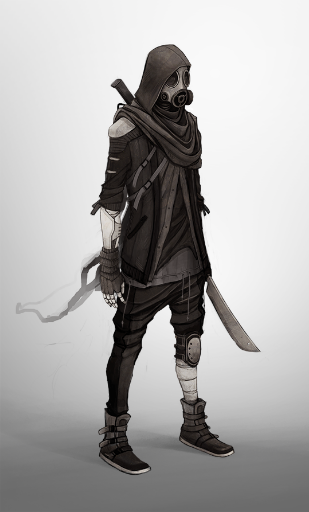
\includegraphics[width=80mm]{./content/img/martin.png}
\begin{figure}[h]
\end{figure}
\end{center}

\textbf{Details}\\
Race: Construct\\
Class: Bard/Sorcerer\\
Age: 87\\
Status: Possibly a Mouse\bigskip

\textbf{Background}\\
The AndelBergers seemed like any other old aristocratic family from Lindedorf, at least from the outside. Who was to know that the family line stretched almost a 1000 years back in history. So far back that the families histories pre-dated the sundering itself.    \medskip

Lord and Lady AndelBergers had been (in)breeding their family ever since the sundering to maintain a pure bloodline, the latest incarnation had proved very difficult indeed as the Lady had only managed to produce a single child, a solitary lady who glowed with the radiance of Hemotate. She was schooled from the families great library and a sense of destiny passed into her. Until one dark and stormy night the church arrived, or at least a part of the church that people only talked about in whispers. Dark masked figures stormed the house and decimated what was left of the family, what happened to the young Ms AndelBerger is still unknown.   \medskip

MarTin was the family butler, built to protect and serve Ms AndelBerger and keep her entertained. He had been fashioned using the knowledge of the ancient family line, his clothes and parts shaped in strange swirling patterns taken from books long useless. On the fateful night the inquisition appeared, Martin was out milking the cows in the freezing rain. He missed the entire saga, only returning to an empty house torn apart at the seems. He rescued his favourite books, and weighed up his options. He had lost everything, but he still had two purposes, to find the young Ms AndelBerger, and to avenge the family line. As possibly the last member of the family line it was now up to him to return the gods to their rightful place within the pantheon.    \medskip

All this was almost a century ago, MarTin has been wandering ever since    \medskip

Unable to die the butler wandered the streets, then the town, then the city, until finally the continent. Until he was chanced upon by a motley crew in an airship....     

\textbf{Personality and Traits}\\
Martin was very depressed, and lacked the spark of power that helps him deal with the day to day drudgery of being immortal. When he discovered the teams goals were to destroy the church he picked himself up only a little bit. It wasn't until he discovered that his ward Ms Andelberger was gone, and ascended to the heavens, that he doubled down and vowed vengeance
Speaks Tikki Tuck, Goblin, and Low Velterran    

\textbf{Relationships}
Martin is forming relationships within the team, he seems most attached to Burnie.\bigskip

\clearpage
\section{Anthony K Tigerius III}

\begin{center}

\includegraphics[width=80mm]{./content/img/toniTiger.jpg}
\begin{figure}[h]
\end{figure}
\end{center}

\subsection*{Details}

Race: DesertCat\\
Class: Barbarian\\
Age: 42\\
Status: Wandering the Expanse with an assassins contract out on him

\subsubsection{Background}

Anthony has been sent from the Guild of Coin in Hopes Rest to open negotiations with one Riphard Obsidian Hardstone.

\subsubsection{Personality and Traits}

Toni saw the possibility of a better world, he did all he could to help ensure that the lessons learned in the desert could help others around him.

\subsubsection{Relationships}

Toni always wanted to work closely with Riphard, who in his mind was an un-tempered prodigy who would take the world by storm. He had big hopes that the power and wealth that Riphard could wield, could be used for the betterment of all in Velterra.\bigskip

\clearpage

\twocolumn
\chapter{Episodes}
\section{Episode 1: Riphard Begins}

\begin{multicols}{2}

\DndDropCapLine{W}elcome to the world of Velterra, domain of the Seven, who rule over all from afar through the constant vigilance of the Church.\medskip

“In Hope’s Rest, the largest city of the Empire of the Seven, a cloaked man dashes over rooftops, a half-burnt tome tucked under one arm as a group of mercenaries chase him. Abruptly he comes to a dead end, a roof with nowhere to leap to and nowhere to hide. He turns to face his attackers and reaches for his weapons, the book slipping from his grasp as he does so. In a moment of panic he spins to grab for the book, losing his balance and toppling from the roof as the mercenaries swing their blades at his back.”\medskip

“In the north, a pair of goblin twins flee the perils of Valkar Varg’s reign, seeking the freedom and new life the south can bring. They are surrounded by brutal tribesmen and vicious axes on all sides, angered by their desertion. As the two goblins look at each other in desperation and anger they nod, the girl raising a long rifle that quivers with electricity, the boy raising a small hunting bow and quickly loosing several arrows. As their enemies close in the bow-user pulls a vial of some mysterious viscous liquid as his twin sister unclips a thrumming round device from her belt. In moments, a huge explosion rips through the area.”\medskip

“To the south, a dwarf pastor sits hunched over a tome, scribbling notes. He raises his head as he hears the slow creak of his door, aware that he is expecting no visitors. He stands and turns to see a hulking figure behind him, armoured with a long-barelled gun at his side. The dwarf rests a trembling hand on his holster as a man who should not exist stands before him. Terse words are exchanged, accusations and threats. The dwarf grits his teeth and sets his feet, drawing the pistol at his side as his opponent does the same. From outside, the sound of a single shot being fired can be heard.”\medskip

“To the East, a figure wrapped in cloth and strange garments sits quietly in a harbour tavern in Port Averdale, recently arrived on the continent from a long voyage. She sits with an untouched mug of unappealing ale in front of her as three thugs approach the table. They slam down a parchment on the table with a picture and a hefty figure. In a flash she is to her feet, blade drawn and two of the men sliced apart on the ground. She faces the remaining thug who whistles and a stream of men pour into the building from all around. Outnumbered by scores and with a demand the surrender, she chooses the only option she knows. Honour.”\medskip

A group of strangers meet up in a featureless, polished stone room, none fully understanding what has brought them there. An elephantine creature (Meredith) beckons them through a mysteriously appearing door into a plush office where a red skinned man wearing a human face mask welcomes them.\medskip

The man explains that he is called Lazarus and that the group have all recently died. They have been brought together, here, and given a second chance at life in exchange for carrying out a mission to destroy the Church Upon asking for proof Pilch is shown the full, gory reality of their situation through a window into hell Lazarus explains that the group must obtain the Stone of Anthala from the temple of XXX and our given basic directions. This ancient relic will be the source of future communications with Lazarus and his means of issuing further instructions. They are warned not to gain the attention of the Church.\medskip

The group agree to carry out the task and are transported into a cavern, where winter clothes and supplies await them. After some brief introductions Exme opens the cave door to reveal they are in a snowy wilderness The group spend two days walking South (Kolo relieves Pilch of 15 gp during the trip) until they reach the town of Vathos Boundary. During a surprise fight with some wolves the two goblins disappear. Riphard finds that his gun has become faulty but is able to restore it to proper working order with a good clean.\medskip
The remaining members enter the town, Pilch in disguise, and go about making inquiries. Riphard and Ontario make a visit to a local smith, not Gerard, who is able to sell bullets and black powder. Onatrio gets the lay of the land, and discovers that the locals are fine with the Church.\medskip

The two goblins, desperate to perform their own investigation and disguised as a single person in an overcoat, put Pilch’s money to work inebriating an entire titty bar, whilst loudly exclaiming their adventurous intentions. Otoria witnesses a man being beaten to death in the street.\medskip

Several towns folk inform the party about the dreaded masked “tikk-tukks” that lie to the South of the town, these are small bear like creatures with face masks.\medskip

The party is reunited in the titty bar. After a brief altercation between Kolo and Pilch concerning some mislocated funds, Exme and Riphard discuss the finer points of owning firearms and Esme is thrilled to get her first real look at a Church gun.\medskip

Ontario and Pilchard Meet a hunter named Gerard who gives a brief description of the location of the temple of Anthala lost in the south. Kolo discovers more about what eats people, and gives Pilchs name as a point of contact. Due to the incredible generosity of Pilch’s money, the group are offered free board at the titty bar and take the opportunity to rest up.\medskip

The next day they make their way out of town. As they leave, an explosion rips through the local stable, decimating several horses and destroying the building. Riphard is unable to identify the source of the explosion, however Kolo is quick to demonstrate the kindness and superiority of Goblin-folk by using the rest of Pilch’s money to compensate the stable owner for the damage. Along with casting wild aspersions to the gathered crowd as to who might be the culprit, ie only group who has access to black powder (Church).\medskip

The group make their way south to the temple...\medskip



\end{multicols}

\vspace*{5mm}

\begin{center}
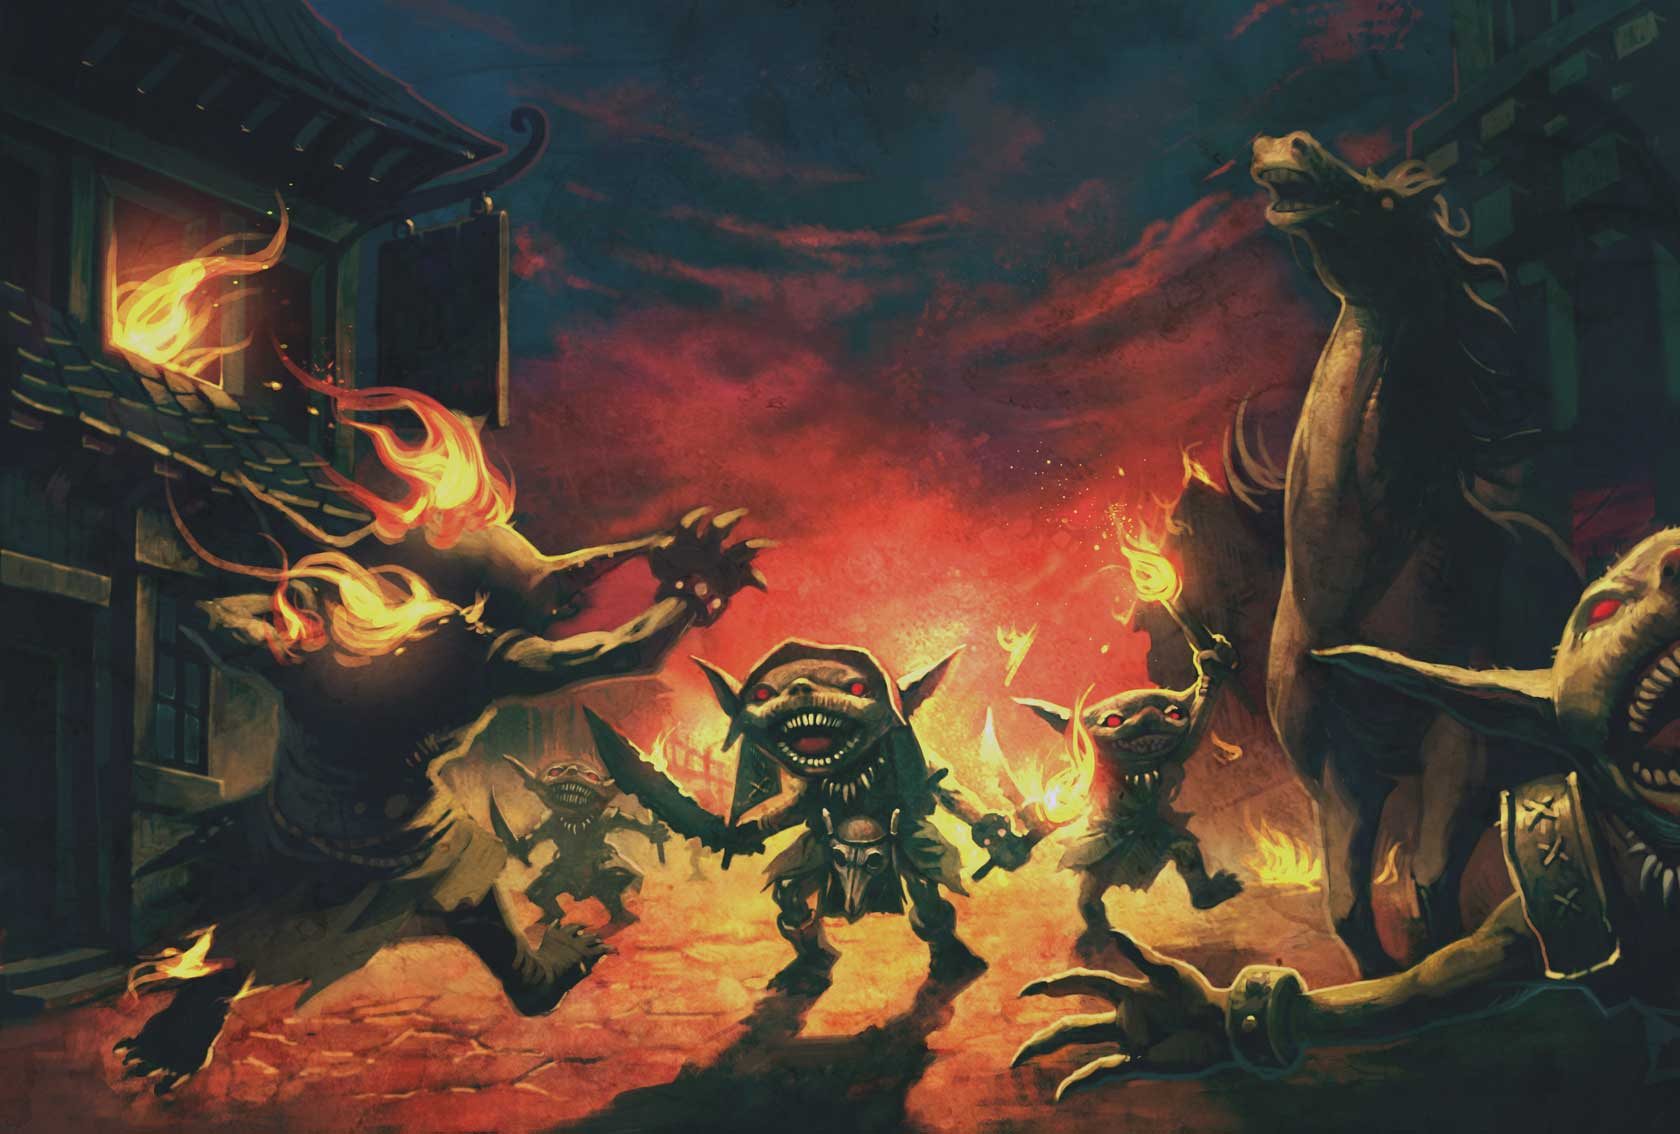
\includegraphics[width=\textwidth]{./content/img/goblin9.jpg}
\begin{figure}[h]
\end{figure}
\end{center}

\clearpage
\subsection{Episode 2: In the Tiki, Tiki, Tiki, Tiki, Tiki Room}

\DndDropCapLine{T}he year is 6653 CC (Church Calendar). In their search for the Stone of Un'thala, the group set off Southwards from Vathos Boundary following the directions given to them by the hunter, Gerard.\medskip

After a day’s travelling the group settle down for the night with Kolo and Pilch taking the first watch. The tension and hatred between the two is palpable and they stare intently at each other. Pilch is briefly distracted, which gives Kolo the chance to disappear. As Pilch desperately searches for his goblin nemesis, Kolo takes the opportunity to attempt to relieve a sleeping Otoria of some of her gold. As he reaches into her pocket Otoria awakes and deals a deadly blow to the goblin, knocking him unconscious.\medskip

Otoria throws the bundle of goblin into his tent, awaking his sister in the process, who mistakenly believes it is her turn to perform lookout duties. She sets down opposite Pilch and resumes the goblin-human stare off. Pilch inquires about Exme’s “gun”, but is not prepared for the onslaught of technical information that Exme is only too glad to discuss. The conversation ends with Pilch being none the wiser, embarrassed by his own vast ignorance. When Exme returns to her tent Kolo has vanished.\medskip

The group push on towards their goal. After some time they arrive at a large skull shaped ice temple that lies across a perilous looking bridge. Exme refuses to enter without her brother and stubbornly resists the efforts of Riphard to carry her along. Otoria takes charge and heads into the temple.\medskip

As the group enter the temple they find themselves in a large spherical chamber, and have their first meeting with the dreaded TikkiTukks™: a race of small bear like creatures with fearsome, culturally insensitive masks. Battle ensues, with the goblins arriving to witness the felling of the final enemy. An investigation of the stone plinth at the centre of the chamber shows that the stone is missing. The goblins remove some masks from the fallen enemies revealing their ghastly faces with sharp, pointed teeth.\medskip

The reassembled group head deeper into the temple in search of the stone. Otoria takes a moment to collect some herbs being cultivated by the TikkiTukks™.\medskip

Kolo unlocks a locked door, which reveals a room full of small boxes that contain some treasure which the group splits up.** Pilch** attempts to reclaim some of the money that he had "misplaced" in the previous session, shamefully accusing the goblins of thievery. Otoria throws him an azure gem to appease him. As the gold is shared out Riphard warns the goblins: “Next time you want your fair share, join the battle at the right time”.\medskip

The goblins attempt to trick another room of TikkiTukks™ by donning masks. Kolo is able to speak in the TikkiTukk™ language. Exme, not knowing of her brothers ability, attempts a bold deception which ultimately backfires when the two are brought to their knees by the devastating attacks from a room full of TikkiTukks™. The group defeat the TikkiTukks™ and enjoy a short rest to recuperate.\medskip

As they continue to explore,** Kolo** pulls Exme back, warning her of a strange tangle of silk threads that hang in a corridor. The group is set upon by a giant spider.** Pilch** is able to set fire to the webbing that covers the walls and ceiling, which keeps the spider at bay, but also traps Otoria on the wrong side of the flames as she delivers her swordy brand of justice. After a short struggle the spider explodes in a mass of ichor.\medskip

Riphard is having gun troubles.\medskip

Continuing on, Riphard activates an ancient trap that fires darts at the group. However, the goblins are not affected since they are of a similar height to the TikkiTukks™; the darts passing harmlessly over them.\medskip

The group manage to fight a large room full of TikkiTukks™, slaughtering their leader (who begins the battle with the glorious war cry ‘tikki tukk doumo arigatou tikki tukk’ ) and claiming his glorious mask as their own. Even with their Tikkitactics and Packtics they are no match for the group.\medskip

Riphard is still having gun troubles.\medskip

The impotent Riphard falls in battle. Kolo kindly revives him whilst pocketing 5 gp, going easy on the man he has no real qualms with yet.\medskip

Further battles ensue. Otaria falls. In a desperate attempt to revive her Exme accidentally punches her in the face, pushing her one step closer to death. Kolo looks on in dismay. Riphard is able to revive her, and the two share a tender moment as he lays his hands on her for “a little too long”.\medskip

Freshly rested the group find a corridor of doors. In full synchronisation, the crew knock down 4 doors only to find, to Kolo’s dismay, more doors inside: “More DOORS. TRICKSY, TRICKSY!!”\medskip

Riphard takes a moment to explore and comes across a fresh water well. He drinks from it and feels the benefits of its cool water, but already feeling 100\% despite the recent battles, does not fully appreciate the benefits the refreshing beverage provides, and so does not share this wisdom with the group.\medskip

The noise of the group knocking/cutting in half doors causes the TikkiTukks™ to bear down upon them.\medskip

Riphard is still still having gun troubles. Exasperated, he makes one last effort and is finally rewarded for his patience and persistence, destroying what once was a young TikkiTukk's™ face in one well placed and devastating shot.\medskip

The group leave one TikkiTukk™ alive to interrogate and help them locate the stone. Whilst passed out, the TikkiTukk™ is tied up and hung upside down. The two goblins don their masks and get ready to intimidate him. Kolo leads the interrogation. The TikkiTukk™ is keen not to die and quickly reveals that the stone is held in the chief’s room. In exchange for the location of the stone of Un'thala, Kolo promises the TikkiTukk™ that he can be the new TikkiTukk™ chief.** Pilch** is also offered as a “sweetener”.\medskip

Kolo is keen to take the prisoner along, but Otoria cryptically states that she is to “have her way with him”. Pilch, greedy for the prisoner’s vitality through his curse attempts to end its life. Otoria is able to block the first blow, but misses the second, which slices open the TikkiTukk’s™ throat. In a cool rage Otoria pins Pilch up against the wall with her large sword and warns him: “I have to work with you, we have shared goals. But you will not do that again”. Pilch is filled with an intense terror at these words.\medskip

The group collect themselves and prepare to head to the chief’s lair to collect their prize

\begin{center}

\includegraphics[width=80mm]{./content/img/kolo2.png}
\begin{figure}[h]
\end{figure}
\end{center}
\subsection{Episode 3: The Horse Whisperer}

The group begin in the bedroooms of the Tiki Tuks after the brutal, and controversial, murder of the "friendly" Tiki Tuk by Philo.\medskip

The goblins, unimpressed with this behaviour and sympathetic to the Tiki Tuks, head towards the treasure room.\medskip

A brief encounter in the water well room see Riphard unsuccessfully attempt to hold Pilch’s head underwater for more details on his violent nature, but Pilch is able to bat him away, swinging his head up in a glorious little mermaid inspired fashion. When asked why he killed the Tiki Tuk, Pilch looks genuinely conflicted.\medskip

Riphard wanders down an unknown corridor, much to Kolo's chagrin. Riphard explains that while Kolo just wants to find the treasure they know about, Riphard wants to find "the treasure that we don't know about”. Riphard is rewarded for his inquisitiveness by finding a stable full of boar and two more Tiki Tuks. Kolo is able to deescalate any possible fight using his language/diplomatic skills, thinking quickly on his feet about an alibi where he is actually visiting his uncle. The goblins laugh at the success of their favourite trick.\medskip

Riphard discovers another large corridor, this one lined with spiked walls and a mossy floor. Exme is able to discern that this used to be a booby-trapped room, however, it has long since fallen into disrepair. However, she does notice the strange fungus growing on the floor and harvests as much as she can along with her brother. Riphard is asked to help, but stubbornly refuses, not being one to do groundwork for such lowly creatures as goblins. Pilch is asked and curiously finds himself accepting the instructions.\medskip

The goblins head to the chief’s rooms. Exme discovers "nothing at all" in a room that she inspects, whilst Kolo recovers a strange, smooth, and intricately engraved stone under a pile of furs in the chief’s bedroom.\medskip

For some reason Pilch decides to argue that this might not be the fancy stone we have been sent here to find. Riphard queries just how many fancy looking stones Pilch thinks Tiki Tuks will have. Exme fumbles through her bag for a while, eventually pulling out a strange device which she passes over the stone. It delivers a small printed out piece of tape in Goblinese which she eyes before confirming that it is indeed the stone of Un’thala. Otoria is not surprised as she feels that most normal stones would not have received such careful treatment and preparation. The goblins inform the group that it is time to sleep, but the rest of the group resist the idea.\medskip

The group take some food from the stores, but are urged by Kolo to leave some for the Tiki Tuks. Kolo also leaves a message saying “nice to see you uncle”.\medskip

Pilch is racist.\medskip

The group travel for half a day, back towards Vathos Boundary, Exme noticeably struggling with her large and heavy bag. The group set up camp. Exme disappears for a short while and returns with herbs that she starts combining with the fungus in a small pestle and mortar. The entire group finds themselves falling asleep.\medskip

During their sleep they share a common dream in which Lazarus speaks to them and congratulates them on their progress so far. He lays out the next challenge, which is to head north to Hope’s Rest. He reveals Pilch perhaps has the closest connection to his kind. He instructs the group that they are to set up base in this liberal township, and will require money and transport to further their interests. The dream fades around the chuckles of Meredith.\medskip

The non-goblins in the group feel weary and drained.** Pilch** deduces that they may be suffering from Zukor’s Rot as a result of being shot with ancient darts in the Temple of Un'thala.\medskip

Exme hands Pilch a single packet of grey paste. She thanks him for his help in gathering the fungus, but berates him for his treatment of the murdered Tiki Tuk.\medskip

The group travel back to town and Otoria begins making inquiries concerning the exploding stable. Kolo and Exme mysteriously disappear. It is revealed that on top of this disaster, the town is now suffering from a spate of horse robberies, including those that led a caravan which is rumoured to be travelling to the north.\medskip

The group visit Black Smith the blacksmith where Kolo, mysteriously reappearing, requests new daggers. Exme, also mysteriously reappearing, attempts to hire the workshop to complete a project. Smith is initially dismissive, however his mind is changed rapidly when offered an ornate, solid gold necklace in return. The goblins begin their work, Exme concentrating hard on her work, and Kolo jumping maniacally on the bellows and hitting things with a hammer. The remaining members head to the titty bar.\medskip

Pilch tries some new, innovative ways of begging - he attempts hawks the Tiki masks as blood money, and gets a free drink from other alt-right extremists, but is told to sell the masks to the captain of the guard.\medskip

Riphard follows the blacksmith home and, once he has gone to bed, breaks into the man’s home and steals the necklace back. The rest of the group is unaware of this.\medskip

The group meet up in the morning and Riphard inquires where to fence sell "totally legitimate jewelry" in the town. He is directed to a jewelry shop where he is given a reduced price for the necklace. Shops have to make a profit, so that is completely normal practice and not a reflection on Riphard's bargaining skills.\medskip

The group head to the city guards offices to inquire about potential jobs and the stable mystery, that isn’t really that much of a mystery when you think about it because it was probably certainly a black powder gang or church related jobby.\medskip

They meet the half orc captain of the guard Urnok and his troll “friend?” Gumshoe. The group discusses local issues and learns more about how they may secure passage to the North.Kolo is a good detective gabrin. Riphard assures people he is a real pastor. Pilch sells 6 Tikki Tuk masks.\medskip

The following jobs are highlighted:\medskip

    Giant boar - Farmsteads in the North offering 50 gp to kill it.\\
    “Jennie’s girls” - Ex-whores who turned to crime after their profession was officially outlawed. Spread like herpes through the empire and can most likely be found to the north. Their leader is a woman called May or “some bitch called May”. The group is told t'arrest her, May.\\
    The SRA - Small Rights Activists. A collection of, mainly, gnomes and halflings who perform terrorists acts in their most-likely justified quest for improving the rights of smaller folk. Leader is Razzle Backshine, a gnome with a penchant for exploding things in people’s faces. Also spread out through empire.\\
    Diego Escabar and his Merry Men - A charming half elf who claims to steal from the rich and give to the poor, but doesn’t actually do the key last bit. Likely located in woodlands nearby. This is a local group.\medskip

Jobs are paid at a going rate of 5gp per severed left ear. Riphard wants to provide scalps, but is informed by Urnok that scalps are too easy to forge. Riphard accepts this explanation, explaining to the group that ears have a unique print, like fingers, which can be compared to the ear-print database the chief almost certainly keeps for this very purpose.\medskip

The gabrins try to turn Pilch in to the guards as Diego, but are unsuccessful. Riphard wonders whether Diego's men would live in a sort-of ghetto, a "robbing hood" if you will.\medskip

Pilch points out that it may be useful to try and recruit these groups, or at least align their interests with our own, and work together against the church.\medskip

Kolo asks Pilch if he has had sex. He replies that he totally has.\medskip

Riphard does not want to arouse suspicion and tries to persuade the group to let him visit the local pastor by himself. After some initial reservations the group allow him several minutes alone before they also insists on seeing the pastor themselves for no discernible reason or purpose.\medskip

Riphard's meeting with the pastor gets off to a tense start. “Are you here to help me?”. “Quite the opposite”. “You’re here to hinder me?”. Riphard questions the pastor on "the inquisition", but the pastor bats away his inquiries as mere tall tales. Riphard attempts to show the pastor proof of the inquisition by showing him the fatal wound he received that sent him to hell, but upon lifting his shirt finds his body shows no signs of trauma at all. The pastor tells Riphard he should ignore these scare stories. Riphard replies that in fact it is the pastor who should not ignore the warning signs. The rest of the group is unaware of this.\medskip

Riphard storms out and walks past the group without a word, looking very pissed off. The group take this as a sign to enter themselves.\medskip

Otoria and Pilch question the pastor, who has suddenly developed a tremendous stutter for some reason, and learn some things about how the Church operates, predominantly linked to their communication channels.\medskip

Riphard looks at boobs, too cheap pious to pay for a touch.\medskip

The group end up in the titty bar where Kolo is able to charm/seduce the busty barkeeper into revealing that she used to know May, back in the day. She reveals that May can be expected to be found to the east of the First River. The lady, flushed with lust towards the sweet-talking Kolo, retires to a back room to cool down. Kolo mysteriously disappears again.\medskip

The group spend a final night in the titty bar before setting off on their next adventure. As they sleep Lazarus visits them again to tell them that now they are in possession of the stone, some members may find themselves more attuned to any pre-existing magical conditions, but that this shouldn't affect their premiums.\medskip

\begin{center}
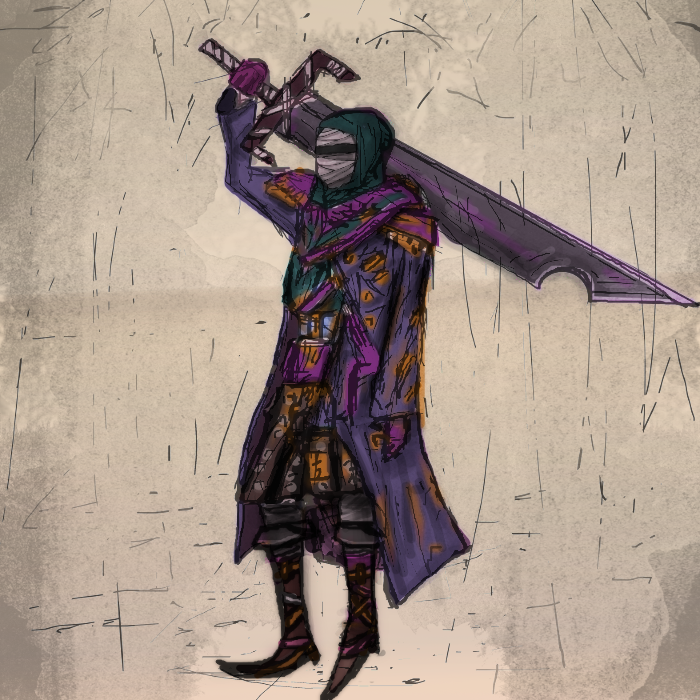
\includegraphics[width=80mm]{./content/img/otoria1.png}
\begin{figure}[h]
\end{figure}
\end{center}

\clearpage
\subsection{Episode 4: Whores or Boars?}

\DndDropCapLine{R}eturning to Vathos Boundary, Otoria and her assorted friends are seeking passage North, and have been given a list of gangs that may have stolen all the horses.\medskip

They wake up in Marcey’s and try to decide how to proceed.\medskip

Otoria wants to infiltrate the Heights Rights lot. Gabrins wants to hassle the Fancy Men.\medskip

Riphard sits in the pub, the Gabrins run off.\medskip

Riphard wants to walk 6 months instead of finding any horses. He sits in the pub by himself to try and achieve this.\medskip

Gabrins and Otoria else goes to see the Blacksmith who’s real sad. Apparently his necklace has got stolen. Otoria wants to find it. They go off to the Blacksmith’s house and look for clues.\medskip

Pilch and Riphard bond.\medskip

CSI:Vathos ensues at Black Smith’s house. Apparently the necklace was stolen by one non-small person. The fidelity of the blacksmith remains in question.\medskip

Kolo looks for criminals to ask questions.\medskip

Riphard is pissed. It’s, like, 12:30. Pilch leaves him to his own demons and goes to wander the streets aimlessly.Then, all of a sudden he discovers something important.\medskip

Meanwhile, or earlier or something, Otoria talks to the police man and he suggests she checks the local jewelers, so see if whoever stole it tried to sell it. She says she’ll have a look.\medskip

Gabrins go into the Mos Eisley Cantena, and talk to a big orc man. Kolo tries to be tough, but is absolutely not that and gets thrown around and nearly thrown out. Then Esme gets involved and is intimidating as fuck. She tries to get the orc man to play cards to win information about the Fancy Man, but that doesn’t work. There’s all sorts of back and forth.\medskip

Then, a “Fancy” Woman appears (not a “Fancy Woman”). She offers to help the Gabrins if they come to their hideout. They say they’re going to gather everyone up and head out with her.\medskip

Pilchard found an old man. He talks to him about how things aren’t as good as they used to be. There’s also not as young a man. Their names are Casper and Germaine. They are woodsmen. He scares them by being a crazy person. There is no inquisition. He asks them if they know any benders. Pilch is a weirdo.\medskip

Otoria finds the jeweler, and the necklace, and the truth.\medskip

Riphard is pissed. Then he’s outside in the alley, propped up against the bins, with Otoria trying to kill him, and then Gabrins trying to steal his money. The Gabrins want to keep him alive, but Riphard himself doesn’t seem to have as much interest in that and tries to shoot Kolo. He misses, and Pilch turns up. Riphard tries to run and is instantly struck down. It’s tragic.\medskip

Otoria starts dragging him to the police station. Half way there she’s convinced to take him the blacksmith’s instead.\medskip

The blacksmith convinces Otoria not to take Riphard to the police, when the group tell him everything, because he would be killed by the church, attracting a lot of attention. Otoria wanted to cut him into little bits, so she’s not super happy about him getting away scot free.\medskip

The group give the blacksmith a shit ton of money, then go back to the pub. Riphard sleeps his pain away.\medskip

Gabrins stack up inside a coat, and everyone goes into the alley to meet the lady.\medskip

The lady is totally fooled by the Gabrins in the coat, for real. She insists on the group helping her or some shit before she tells them where the fancy men are.\medskip

The group head North, out of town, to Whorecity. Then west, then through some hills, then some hillocks. Then there’s a camp. It’s a little bit secret. Otoria and the lady (who’s called Delilah) get on like a horse on fire (like what happened in the stables that time).\medskip

WELCOME TO WHORECITY!\medskip

The group get taken to the Queen Whore, Mae. They brag about their wealth, insult Mae’s fashion sense and then finally get round to actually talking about why they’re there.\medskip

Djago and Mae don’t seem like besties, but Delilah jokes that they are. What’s up with that?\medskip

Exme wants to know what whoring is.\medskip

Otoria wants to know where the horses are. Mae implies, but does not say, that she knows where they are, but says they need to do work for her first.\medskip

Kolo makes a deal. No one’s quite sure what it is.\medskip

Apparently the whores buys their boots in bulk. They’re damn fine boots. We should get some.\medskip

Mae admits the Fancy Men have all the horses, and says she’ll tell them where to find the Heights Rights lot, so they can kill them, and then she’ll tell them we’re the Fancy Men are, so that they can kill them.\medskip

Otoria tells Mae not to tell anyone they’re there. Esme tells Mae that they’re terrorists planning to take down the state.\medskip

Everything seems fine.\medskip

Mae has work to plan.\medskip

The gang manage to get two horses, and squeeze on to the back of them.\medskip

Riphard gets hit on\medskip

They ride horses to Razzle’s house. Razzle is king of the Height Rights. This is his house.\medskip

Gabrins are going to go in first, like they’re HeightRightsers. They’re going to see if they can find Razzle, and then come back and do some Strats and Tats.\medskip

Gabrins enter HeightRightsManor.\medskip

There’s a fucking hobbit.\medskip

He’s going to fucking whistle like a bellend.\medskip

The Gabrins shout at him and introduce themselves, to get ahead of the scandal.\medskip

The fucking hobbit’s called Nickles.\medskip

“Big rights for small people”, says Esme.\medskip

The Gabrins tell Nickles that they’ve been persecuted for being little. Kolo has terrible flashbacks to the Cantena. This pleases Nickles and they get taken inside.\medskip

I can’t really see what’s going on any more.\medskip

There’s a sleeping area and some stairs.\medskip

Here’s Razzle. He’s a gnome. He’s got a big bag of fireworks. He’s stressful to listen to.\medskip

He’s a little leprechaun gangsta, see.\medskip

He wants to burn Djago down, see.\medskip

Esme tells everyone about wanting to bring down the church again. Razzle wants to kill humans indiscriminately. It’s a debate for the ages. Only Razzle can use the boomstick.\medskip

Esme’s, like “please”. Razzle’s like, “NO”.\medskip

Esme offers information about booms, in return for… a thing… or… anything. Hundreds of short people will die, but I think that’s the plan. I really don’t understand. It definitely sounds like they’re not going to kill this guy.\medskip

Razzle wants Gabrins to kill whores.\medskip

Razzle wants to be quiet and small. He’s failing at half of that.\medskip

Kolo wants to pick up part time job killing humans, Esme thinks they should focus on taking down church, so that they can kill even more humans.\medskip

Gabrins suggest Razzle should come with them on mission to kill whores. Razzle says no. He sends his best men, though.\medskip

The Gabrins and the best men go out into the woods, where the Bargins plan to kill them. Otoria and Pilch talk about when to kill everyone.\medskip

They eventually decide to wait until everyone’s asleep.\medskip

In the woods, everyone’s asleep. Time to die.\medskip

Pilch tries to back out of this whole thing, trying to get the Whores and Height Right’s to be friends.\medskip

Otoria wants to cut off their tongues and hands.\medskip

Esme is spread the gospel of The One, trying to convert the Best Men. Esme and the Best Man (who’s a woman) take a minute and pray to The One.\medskip

Everyone else is hanging out in the bushes.\medskip

Everyone suddenly doesn’t want to kill them any more. They feel really bad for the small people, but then they kill them anyway.\medskip

There’s a brutal massacre.\medskip

Everyone decides that they’re going to kill Razzle, but that they want the small people to be free and happy under a new ruler.\medskip

Everyone gets back to the cave and prepare for shit to go down.\medskip

TO BE CONTINUED...
\subsection{Episode 5: Pitter Patter of Tiny Bears}

[The following pages are torn from a larger volume, and hastily rebound with string - One corner is singed implying someone attempted to burn this or the entire volume.\\
The writing is in a quick, hurried, but practiced hand, and the type-face changes occasionally as though the writer grew bored of their style]\\
Codenames as follows...\\
- SH - Shadow Hound - Yours truly\\
- RP - Righteously Pissed - the drunken dwarf\\
- JR - Jilted Royal - the foreign lady\\
- SR - Shifty Rogue - the thieving goblin\\
- JM - Joyful Mechanic - the inventive goblin\\
\DndDropCapLine{S}o we’re in a cave, and just slaughtered a small number of small folk to whom we hope to ally. Great.
SR has initiated a plan to take over the small-peeps by killing Razzle, SH says we should try and discredit the small folks leader (Razzle) - Seems that the goblins and Dwarf are going to go in and try to convince everyone else that he’s gone rogue and isn’t part of the organisation anymore.\medskip
I’m loath to split the party, but the tiny bigots (...small-ots?) probably won’t like me or JR walking in - maybe we can be guards or sympathisers?\medskip
Anyway, I do the honorable thing of burning the bodies (and taking 5 ears), and then forging a document for RP -
"Razzle is accused of collusion against the SRA with his Ofecal Cherch Buziness."\\
We stop outside, and finalise the plan - is as above, but the goblins will go in shortly afterwards to make it seem they were (recently) ambushed.\\
RP Successfully enters the camp, thanks to the forged letter. The goblins sneak in after. RP manages to get found as an imposter, despite the letter. He did not know the secret Nichols handshake.\\
A fight breaks out between RP and 3 members of the SRA - but he’s quickly subdued.\\
Everyone decides to scapegoat RP as a church-worker, still to discredit Razzle. Goblins sneak in.\\
SRA becomes SRM - suddenly, because RP.\\
Goblins come in, pretending to be injured - leant huge credence by my amazing disguising. Two of the SRA fall for it.\\
RP gets blown up. Probably. Razzle likes bombs. “No dwarfy… I expect you to die!”\\
RP starts whipping people. He gets knocked out.\\
Team gobbo and 2 of the SRA run in. One gets blown up, the rest like Razzle more for this.\\
JR is very noisy, it messes up our stealthiness.\\
SH becomes a rock.\\
I get RP back up by punching him, and then dance like my life depends on it (which it did).\\
RP is then useful by disarming Razzle.\\
Razzle Shanks me, but the shadows protect.\\
The JM Blows off Razzles head.\\
SH, RP and JR (who had been doing pull-ups the whole time) leave.\\
The goblins appoint “Buttons” as the new leader of (this faction) of the SRA.\\
There's maybe 4 SRA left.\\
They also loot: Signet ring (with stampy well) 10 rockets 10gp\\
Papers - Bits of communication, Old Plans, Promotional Material, rambling letters,\\
I’m not happy about this.\\
We rest up.\\
Kolo and Otario have a heart to heart.\\
We all go to see Mae. JR takes point in the conversation. It’s interesting. Mae and Delilah plan with us to go kill fancy-pants.\\
I’m on a horse.\\
Mae gives us 3 people to go take on Fancy-Pants, Diago. One is an Battle-axe barbarian type, others a Crossbow-marksman, as is Delilah.\\
JR and JM also get fancy “dutty ho” boots.\\
On the way (to Diago) we encounter a man that tells us about the giant boar. Delilah flirts with RP for some reason.\medskip

JR - with her Mechanism Bow, JM and SR decide to attack at ranged, and take out the boar slowly.
In the forest, we get attacked by dropbears.\\
RP gets ripped hard. JR flails.\\
Me and the goblins kill nearly everything.\\
The crossbow whore (Martha) dies.\\
I save RP.\\
I get Martha’s Xbow.\\
Wait, shit… I better burn these pages - safer than leaving a paper trail... \\
\begin{center}
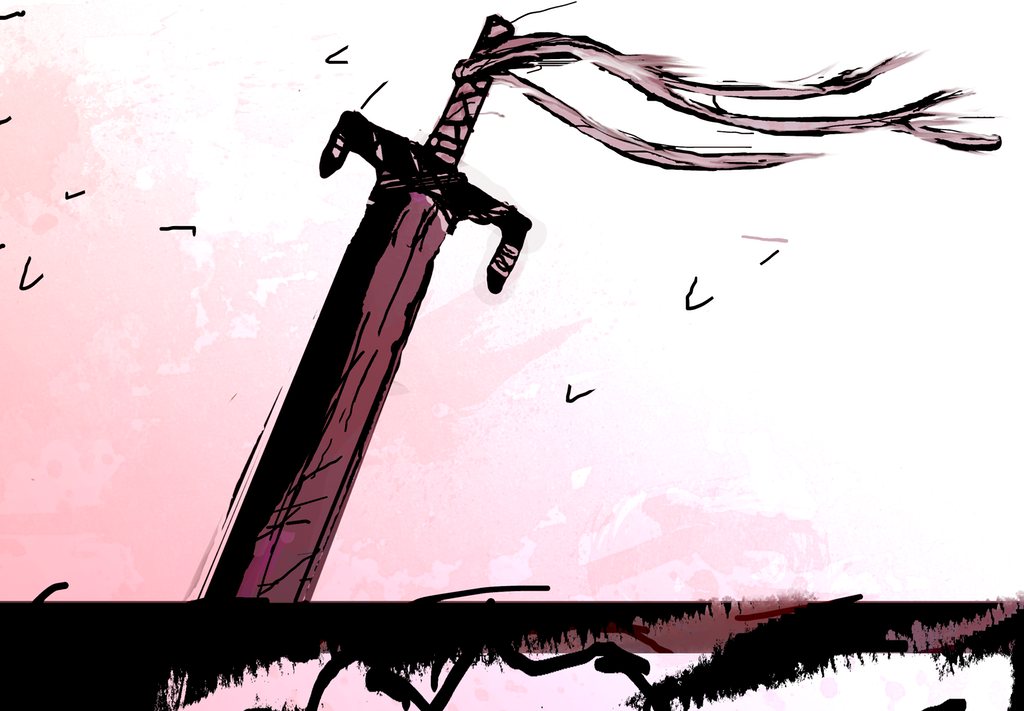
\includegraphics[width=80mm]{./content/img/otoriagrave.png}
\begin{figure}[h]
\end{figure}
\end{center}

\clearpage
\subsection{Episode 6: Arbitration}
\DndDropCapLine{D}ay starts well as we are unmolested\medskip
Pilch talks to Delilah about other men and how to lure them in, he is very keen even if it means traversing vast tracks of forest. Even the Dutty Hoe isn’t willing to put out that far.\medskip
Camp is made, no one wants to sleep, perhaps everyone is super excited about meeting the giant pig. Kolo gets bored and falls asleep.\medskip
Fishy loses his bird, Kolo helpfully brings it back, but it somehow escapes. I am intensely interested in how the bird works, could be proper useful to have a scout, and something to distract enemies in a fight……\medskip
Fishy will pay for this, but first I follow Pig Smells.\medskip
Otario and I go for sneaky first kill on Pig, which is followed by a sudden tactical climb into a tree. Otario winds up and pitches the Gabrin Fast Ball Special. Negotiations unfortunately fail, and after bouncing off the pig… watches as the Strange One leaps and pirouettes onto the big piggy before spanking it with her giant sword.\medskip
Exmeh then lines up a shot and whispers "This little piggy went to market" before dispatching one baby pig.\medskip
Before suddenly there are two Exmehs, wandering about. The Evil twin Exmeh then kills poor little piggy No 2.\medskip
Riphard blows Big Pigs brains out everywhere, no more piggies.\medskip
“It is Impossible to have a Cake and Also eat a Cake” Strange on is Strange.\medskip
Barbeque pork all around, as Pilch adds to his ear collection. Big Pig is Too Big except for fatty hoe who eats most of pig. Impressive…. Riphard is strangely not interested in pig.\medskip
After camping overnight in the pigs den, we move on to through the woods following filthy hoe Delilah. Somehow she knows where fancy man lives….\medskip
Pilch watches Kolo taking a massive smelly pig sized shit. About half way through, kolo turns and make eye contact while pinching off the end of the loaf.\medskip
Pilch is confused about horses and dirt hoes.\medskip
Its agreed that all ravens will now be shot.\medskip
Pilch is a huuuge fiilltthhhyyy liar, about where the enemy are and what they are up to.\medskip
Otario leads the lady charge, to entrap the fancy men. While we sneaky for horses, except Riphard who walks into the camp bringing the good news of the lord.\medskip
Things go well with the fancy pants, as Otario works her magic\medskip
Kolo horse whispers with his own shit, and as he is tying up the horses, stoooopid Exmeh sets off a fire work. Otario then starts a song and does the dance of her people, it is not impressive.\medskip
Exmeh stands statue of liberty esque holding a boom stick high.\medskip
Kolo sets off a horsey train through the camp. “ A sudden Rampage “\medskip
One bandit does his best to salve the horses, “I’ve got this lads” by running in front of them all, who then savagely kill him.\medskip
Otario gets Axed a lot of questions, while pilch hides behind a tent and tries to convince the fancy men their leader is a nerd. Riphard starts a loaded sermon. Exmeh sends some redundant technology burning some poor fuckers face off, before hiding behind a tent!\medskip
Pilch finally finds his ball sack, no correction he hides behind another tent before trying to reason with the enemy again. Luckily he is saved by the tent catching arrows. Strange booyagh is afoot as voices from the forest, as the horses speed out of the village.\medskip
Raven hunt is going very badly, something is definitely up with this freaking bird. Its naked.\medskip
Pilch somehow convinces half the archers to go to bed, while he gets nailed by Capn’ Fancy Pants, and leaking smoke.\medskip
Otario is taking a nap on the table, while Pilch makes an ill timed verbal foray against Capn’ Fancy Pants, and as he pulls out his knife his chest explodes across across pilch from Exmehs rail gun.\medskip
Riphard finally deals with the pesky Axe man, blowing the back of his head out.\medskip
Sterling doesn’t make the cut because Kolo makes the world a better place with one less asshole. Pilch cuts more ears from Diegos Boys, chopping Diegos head off for good measure.\medskip
Otario rides off into the sunset badly, Delilah suddenly decides to stick with the party. Possibly because of sexy smelly gabrins.\medskip
Pilch gets some hot whispers from mega Hoe.\medskip
Return to sender, to find some poor mug still getting a shoein.\medskip
In the middle of town we discover a plate armoured individual standing over a leather clad man. She is holding a gun to the mans head. The gun is bigger and badder than Riphards, giving Riphard a massive Hard on.\medskip
Kolo shits himself, Otario tries to take the hit, but then Riphard out of nowhere gets the game on with the Arbiter! Truth will come and Justice is serverd liberally with a massive sword.\medskip
Otario and Riphard are totally outclassed. Otario gives a long winded speach to the crowd, while Pilch is gone, and the Gabrins are at the titty bar. It doesn’t quite go the way she planned. Not even able to take out a wooden pillar afterwards. She then stalks the scary arbiter woman.\medskip
Riphard gets some top tips from the Scary lady. Otario gets a letter for 500 gold from Arbiter Kyross, which she lets drop to the floor to be cashed at Rivers Falls.\medskip
Riphard gets a note, recommending him to the master at Rivers Falls. To train him up with ninjas. The idea of training with the Ninjas makes him cry. Its genuinely touching. He also pockets the 500 gold note.\medskip
Otario continues to stalk Lady Kyross, throughout the day and night.
\subsection{Episode 7: Mysterious Incident of the Cow in the night}
\DndDropCapLine{P}ilch is the anonymous Jackalope, also in attendance is Anonymous Hippo and Anonymous Frog\medskip
Hester is the owner of the caravan\medskip
Otario is found in the town still staring at the kebab ladies house. He agrees to meet everyone at the main square for departure. In the mean time Otario pays a small urchin to send a letter everyday to convince the Kebab lady that she is still watching her\medskip
At the caravan Kolo is upset that everyone has a caravan except for him. Exmeh locks him out. Pilch cosies up to Hestor\medskip
Boamos under represented caravan member that Otario befriends. He is from South West Africa, which no one has ever heard of. He is happy to help learn Otario. “Otario learns horsecraft” its super effective.\medskip
Riphard and Delilah are having a muffled “conversation”\medskip
Kolo pissing into Exmehs caravan, before running off with tongs and a crucible.\medskip
Pilch looks for some general information, specifically against the church. Exposition dump, nothing out of the ordinary other than that constant war with the minons of the (Valkaar) VARG, and those from Lindedorf who are striking back at the church.\medskip
Caravan People Consist of:\medskip
Leader: Hestor\medskip
Guards: Leorable, Dukey, Dallius, Job\medskip
Merchants: Boamos, Tillie, Sabina, Maarah, Sidney\medskip
Troubles in port AbbeyDale in the East, more people from Masooda, Far to the East across the Ocean. Masooda and NanDuan are not friends.\medskip
Story time commences, involving Drop Bears and changelings….\medskip
Changelings are revealed by throwing salt over their right shoulder...\medskip
NanDuan has a plethora of sand daggers\medskip
Otario makes friends with a horse, before …\medskip
Kolo goes off for a stealth investigation\medskip
Pilch is caught spooning Hestor\medskip
Fierce discussion takes place about what to do about the ambush. Pilch wants to hide in the, kolo is a fan of stalking the beast\medskip
Pilch has not romanced Hestor after all.\medskip
Hoof prints are massive, but its super light on its feet.\medskip
Probably one of the Nanduisian Balloon Cows\medskip
Otario and Kolo join forces and become Super Mega KolOtariozord, its is not supereffective\medskip
Everyone runs blindly into the woods, some more blindly than others\medskip
Otario prepares the bey blade, but to no avail as she is booted out from underneath kolo, but what is not a flying cow afterall.\medskip
Pilch runs away leaving otario and kolo to die. Luckily the Leucrotta is slain by Riphard awesome boom sticks, and the cross bow bolt of a returning Pilch.\medskip
Exmeh fixes up the axle of the lead wagon and the party moves onto RiverFall which is beautiful.\medskip
In the middle of which is a large church, the sanctuary of Novetta.\medskip
The spire of “emoticon” -Imota Kan\medskip
Riphard hates women\medskip
Armor is expensive
\subsection{Episode 8: Freaky Fishy}
\DndDropCapLine{A}s we join our “heroes”, they have just arrived in the town of Rivers Run or something. It was a long night, so a nice warm burrow was dug for Pilch to enjoy. Pilch lives in a hole in the ground.\\
This town that they’re in is where the church lives.\\
People really want Otoria to stop dying so much and actually help, so they’ve all gone to the shop.\\
They can’t afford any armour, so try to find work to get money. Apparently there’s trouble a’ mine.\\
There’s a bunch of other places to go too.\\
And 4 taverns. Rip gets hard.\\
Sad Crusader, Club and Cask, Open Flask, Minstrels\\
Sanctuary of Novotel - Church place to gain power and money\\
Everyone goes to the Sad Crusader, obvs.\\
It’s great. Everyone has a good time and the service is great.\\
Kolo burns the raven.\\
Pilch drinks terrible beer and Kolo drinks some Killepitsch shit.\\
Kolo buys some of it and some matches. There’s no explanation for this at all.\\
Pilch goes wrong somehow and starts rolling around in his own vomit.\\
Everyone decides it’s probably for the best if they put him down, which is sad, but unavoidable.\\
Then Pilch shits magical darkness and Kolo sets fire to the pub in response.\\
Everything goes to shit and people are running through walls and shit.\\
Outside, everyone realises Pilch is possessed or something and start taking him to the river to drown.\\
Otoria realises there’s two old men trapped inside and runs back in to save them. It’s awesome and she picks them both up and bursts out through the wall of the burning pub.\\
She then returns to the rest and helps them throw Pilch in a river. Kolo’s been rolling him, which is cool but not that efficient.\\
Pilch immediately starts drowning. Everyone’s “really upset”.\\
Pilch wakes up and gets out, then he and Kolo mud wrestle for a bit.\\
The fire’s really getting going now, most of the crew help out, Riphard runs off to another pub, Munchkins, the suave place.\\
He doesn’t get let in, because he’s not cool enough, but then he does the classic Inspector Routine, and totally bosses it.\\
He’s in.\\
Everyone else is saving lives and property from that fire they started, but whatever Riphard, you do your own thing.\\
Munchkins is like that cool jazz bar in Spiderman 3.\\
This whole sequence is basically just Riphard’s methdream. Everyone keeps giving him compliments, booze and boobs.\\
Meanwhile, at the disaster zone, the brave volunteers have sated the fire.\\
Otoria gives the man some money for rebuilding the pub and Kolo asks him to come with them on the adventure. He declines, but gives Kolo the recipe for the Killepitsch stuff.\\
Otoria and Kolo take Pilch off towards the Spire of Emoticon/Immodium, apparently Kolo knows some secret Gabrin magic to fix Pilch which seems to involve leaving him in a hole in the ground and leaving.\\
Riphard is 13 shots down. The remaining 7 shots get put in 2 cocktails for the road, and he crawls off to the central church place to report in with what he found from drinking all of this bullshit. It takes him hours.\\
He’s greeted by two guards, he tries to make them drink the remaining cocktails, and then forgets he’s not a female arbiter. Somehow he gets let inside.\\
He’s going to meet the guy who’s supposed to give him all the money. Everyone’s being nice to him, despite the fact he’s a fucking mess.\\
Riphard meets the guy. Gendry goes and gets the money.\\
Riphard tries to hold a conversation. It goes as well as you’d expect.\\
The guy makes him undrunk. He gets nuzzled.\\
Riphard puts his hand on a ball and it tells him his destiny. His destiny is to be an Alligator.\\
The guy tells Riphard to go and pray at some artifact at the Spire, which is run by the guy’s daughter.\\
Gendry does some top-shelf slapstick with a big sack of money.\\
Riphard takes his comical bag of money into town and looks for somewhere to hide it. He goes to an old man’s shit brick house.\\
The old man thinks Riphard is here to put him down. He’s mildly upset about this, but seems to think his daughter would approve.\\
He’s so old.\\
SO OLD.\\
SO LONELY AND SAD.\\
His daughter wants him to die, because she lives in a wooden house.\\
Rip goes off to find a hiding place for his huge bag of gold. I think he’s going to kill this sad old man.\\
He tells the old man that the gods want to run a shop in his house. The man loves this idea.\\
The old man decides to leave his house to the church when he dies. Riphard is definitely going to kill him now.\\
The old man’s name is Derek Bobacious.\\
Riphard goes off the get himself written into Derek’s will. Hero.\\
Kolo and Otoria are digging a hole in the woods. Otoria finds out that Kolo’s planning the kill Pilch before they bury him, and she doesn’t like this. She convinces him to take him to the Spire instead and they ride off.\\
Back in town, Riphard’s got the contracts drawn up, meets Delilah. He decides to take her to meet Derek.\\
Derek gets the will and sexually harasses Delilah.\\
Derek boasts about his old man dick.\\
Riphard opens a bank in Derek’s house. He calls it Northern Rock, because it sounds sturdy and dependable.\\
Derek reveals that his actual old man dick is broken, but the old man dick in his mind is doing just fine.\\
Riphard sets everything up and rides off to meet the others.\\
They arrive at the Spire.\\
They meet Holly. She lets them in.\\
There’s a party going on, but they’re not invited, especially the definitely naturally ill guy they’re here to find a cure for.\\
Riphard presses Holly for info about the vaults and shit.\\
He tries to get investment into a colab on this banking startup he’s planning.\\
Holly tells them where all the books they want are, and also that only Pilch can read the ones on possession and Devil shit, which why would they even need that, because he’s just got food poisoning or something.\\
Riphard finds a book about the thing he’s looking for. Otoria finds a book about syphilis. Kolo finds a book about possession and what to do about it.\\
We need to get a pastor to do a thing and then purge him.\\
If this doesn’t work, we’ll just kill him.\\
We’re gonna fix fishy,\\
Riphard is chanting, Kolo feeds Pilch half a bottle of Killepitsch.\\
Vomit.\\
Vomit. Vomit. Vomit.\\
VOMIT.\\
VOMIIIIT.\\
VVV OOO MMM III TTT\\
It seems moderately successful. Fishy lives.\\
He gets a shadow sword, and stops being so obviously possessed.\\
Pilch agrees to stay at least 15 feet from Otoria at all times he's not actively saving her life, on pain of sword.\\
Everyone goes to a party.\\
There’s all sorts of people at the party, including people from the same continent as Otoria, which is rare.\\
Otoria introduces everyone to a plant expert, and goes off to get drinks.\\
Holly turns back up, and offers to show Riphard the artefact he’s here to see. The others can come too.\\
Pilch puts a sword in his ear.\\
Rip, Kolo and Esme go to see the thing.\\
Pilch goes to be sick in a hole.\\
No one realises that the last time they saw Otoria, she was off getting them drinks.\\
Everyone else is in the vaults, having a lovely time all together.\\
They go and see the thing. It’s a ruby sphere 2 fists wide.\\
Mike loves getting fisted.\\
Riphard meditates into the stone. He realises he loves the church loads.\\
Suddenly, off in the distance, some people hear a scream, most people do not.\\
TO BE CONTINUED
\subsection{Episode 9: Live Free or R.I.P. Hard (In loving memory of Lady Otoria Hearthrust)}
\DndDropCapLine{T}he screaming continues.\\
Holly: “what what whaaaa?!”\\
Holly runs to the door: “Leroyyyy mmmmmJeeennnnkinnnnsssss”\\
The group crowds around the door. Clanking machinery and voices are heard in the distance\\
Man 1 “Tony, we need to break the door down quickly.”\\
Tony (probably) “Don’t worry, she knows what she’s doing”\\
They don’t know the doors are unlocked to this super secure facility.\\
Esme is confused about everything.\\
We open the door and see 3 stunned figures outside the door: burly black man (Theo), half orc (Tony), and Eastern looking lady with daggers. They draw their weapons.\\
MEANWHILE\\
Otoria explores the upper levels carrying around the 3 drinks she got for the group. She reflects on the peace and quiet: that is never a good thing. She hears heavy footsteps bound up the stairs.\\
Otoria freezes and watches the doorway to the stairs.\\
Man 3 “Round up the others. Take care of the hostages, right Alexander?”\\
Man 4 (gruff voice) “Don’t tell me how to do my work.”\\
Otoria approaches Alexander and scolds him for mistreating Man 4.\\
The men note Otoria’s notable weaponry and draw weapons.\\
MEANWHILE\\
Exme is fucking on it and pops a shot off first. She misses.\\
The dagger lady “eyes up Kolo” and waits. Lustfully.\\
Tony gets a glancing spear blow on Kolo (more innuendo).\\
The dagger lady now stabs Kolo for some reason who cries out for Exme’s help.\\
Everyone misses everyone else.\\
MEANWHILE\\
Otoria gets wet for some reason.\\
MEANWHILE\\
Pilch tries to use his new sword. He sucks as expected. He tries to retcon it with luck, forgetting AGAIN about his raven that magically gives everyone advantage. He now magically hits here for minimum damage, giving her the equivalent of a paper cut. Some magical extra damage comes out of nowhere and she explodes. That’s a bad paper cut.\\
MEANWHILE\\
Alexander tries to spear Otoria and bang her (... come on). He fucking rapes her (not litereally). Otoria is in bad shape.\\
Otoria respond with a fancy sword swipe. It’s pretty fucking fancy. The men look impressed and injured.\\
MEANWHILE\\
Riphard talks to his bullets. For 6 seconds. You’d have thought he could manage more than that, but no.\\
Exme kills Theo.\\
“Frank” (Tony?) takes Holly hostages and backs away threatening to kill her if we move.\\
MEANWHILE\\
Otoria continues to battle the two men without dying, which is an improvement.\\
MEANWHILE\\
Pilch thinks about taking off Holly’s clothes. Very inappropriate for an unconscious hostage. Probably telling of his character. Pilch does something involving magic. It didn’t seem important.\\
MEANWHILE\\
One of the dudes tries to bang Otoria again, but misses so badly he makes it super easy for Otoria to stab him. Otoria misses. But in her miss scares the fuck out of the men. They literally shit their pants. Then she remembers she actually had advantage and they retroactively take damage, probably from the pant shitting. The guy drops his weapon.\\
MEANWHILE\\
A large inky black void has surrounded the doorway, pilch, and the hostage situation. This is probably Pilch’s fault.\\
Riphard says “Fuck this noise again” and pats Kolo on the head 10 times.\\
Exme and Kolo looks at each other and realise their opportunity. A vault full of invaluable secrets, during a robbery, with the keeper conveniently unconscious and subdued.... It would terrible if some of the items went missing.\\
Exme uses her identify machine, but it beeps confusedly at her. She walks off.\\
Frank (the girl was Tony all along) panics and drops Holly in the black shit mist. He runs in the direction he thinks the stairs are in.\\
Kolo runs into the black shit mist for some reason. He trips over Holly and falls on his face.\\
MEANWHILE\\
The lady tries to stab Otoria… and misses. The battle rages on.\\
MEANWHILE\\
Pilch reabsorbs the darkness into his ass. He approaches Kolo and offers him a hand to his feet. Kolo thanks fishy.\\
MEANWHILE\\
Alexander runs off allowing Otoria to stab him. She misses. Otoria tries to intimidate the already scared man, commanding him the halt. He stops. Fucking Jedi shit. Otoria then swipes at the lady and she’s barely standing on her feet, crumpling her breastplate.\\
Riphard commands the running man to DANCE! He stops and starts dancing, telling the others to subdue him.\\
Exme is homing in on something and finds a small ring.\\
Frank continues to dance aggressively and sexually.\\
Kolo wants Pilch to throw him and jumps into his arms.\\
MEANWHILE\\
The lady tries to stab Otoria again. Misses again.\\
MEANWHILE\\
Pilch runs with Kolo and throws him at the now stationary and non-dancing Frank. Pilch uses some kind of homing device and bullseyes Kolo into Frank’s face.\\
Kolo does a barrel roll in the air and headbutts Frank while stabbing him, knocking Frank out cold.\\
MEANWHILE\\
The mighty battles draws to an inevitable conclusion. Otoria does some more unnecessary. fancy sword shit and opens some sardines. She cuts the ladies face off and struts towards the still terrified man.\\
“Everything went much better for you because you did what I say. It will continue to be better for you if you continue to do what I do. Tell me everything”.\\
The terrified man spits blood and tells Otoria that they were robbing the place (no shit).\\
Otoria wonders if the man parties. He does. He tells her they took the party people hostage. He says they didn’t want violence, despite rushing Otoria immediately on sight. He said she looked like a badass. Otoria tells him to go to bed and rethink his life. Settle down. Get a job. Contribute productively to society. He agrees to have a nap and try to figure his life out. Otoria breaks his spear and lets him be.\\
“By the way, never seen a woman fight like you.”\\
“I am Otoria Hea…”\\
“LET ME FINISH…. Except for Lark”\\
“Thanks for the cryptic clue.”\\
“No, you already know who that is. The blonde asian lady.”\\
“Ohhhhh yeeeaaaaah.”\\
MEANWHILE\\
Riphard practices his bondage techniques, convincing the others not to skin the man.\\
Exme quickly works out how the fancy 17 lock door works for Riphard.\\
Kolo agrees to guard the treasures (yeah….).\\
The group take the unconscious Frank and now-conscious Holly to the security HQ within the tower, which is apparently just the guards at the door.\\
Riphard explains to Holly about the robbery and non-so-subtly implies the need for a reward.\\
The guards, who have no fucking idea what’s going on at this super secure treasure tower, inquire as to what’s going on. Pilch tries to explain to the guards what’s happening despite all this being Riphard’s idea. Who is oddly quiet, scribbling notes, probably about their lax security procedures.\\
It turns out that the 2 guards are part of the robbery. This explains a lot. Riphard takes notes harder. “TRUSTWORTHY GUARDS!!!!”.\\
Riphard quick draws his pistol and shouts “THUNDERCUNT!” and shoots one of the motherfuckers.\\
Kolo hears the distant rumble of Riphard’s gun. Exme does not.\\
One of the guards doesn’t hit Riphard.\\
Pilch drops an ear (wtf) and further confirms himself to be very much a Stephen character by looking for the best way to run away. He contemplates jumping into shit to surrounding himself with matter similar to himself. Holly and the unconscious half orc block the corridor. Pilch stabs the unconscious half orc to Riphards confusion.\\
Riphard misses with his whip.\\
The men stab Pilch in the face with a greatsword and miss with another.\\
Pilch tries to actually do something useful and stab the dudes (totally after sending the Raven out for advantage). AND MISSES LIKE A CUNT.\\
MEANWHILE\\
Otoria eats some grey goo, totally oblivious to the thunderous blast from below. She decides it’s party time and descends to the party room.\\
The group uncover the mystery of Imota Kan (NAKATOMI BACKWARDS OMG) and it turns out the whole thing is a Die Hard rip off. Pretty sweet. All the dudes are named after the Die Hard people too. Fuck. Does that mean it’s Christmas?\\
Hans (come on) cuts a guy's head off as Otoria enters the room. Everyone starts making Die Hard references.\\
Otoria banters with Hans. There’s a lot of talk of mess and shit shows. No one likes mess. Hans explains he’s here to rob the tower (YEAH WE GET IT). Turns out Hans threw the party in his own honour, what a cunt. The conversation goes on for a while in true hollywood style with the villain fully explaining his plan for some reason.\\
Otoria tries to convince Hans that his men in the vault are dead. Hans proposes a bet to see who’s dead.\\
MEANWHILE\\
Riphard starts singing Firework by Katy Perry, who totally exists in this universe, inspiring Pilch and Holly.\\
The evil dudes miss.\\
Pilch kills a motherfucker and kicks him off the bridge.\\
Riphard fucking whips the other dude’s feet, who entangled in whip stumbles off the bridge to his grizzly doom. Wilhelm scream\\
MEANWHILE\\
Otoria notices Kolo and Exme sneaking out from the all too convenient poop-chutes-come-ventilation shafts. They now know what it’s like to be TV dinners… after they’ve been digested, shat out, and flushed away.\\
The hollywood conversation continues. Otoria tries to walk away, but the henchmen fire their crossbows at her, but all miss leaving an Otoria shaped arrangement in the wall behind her.\\
Exme left a crate conveniently in the party hall last week, which now starts beeping and humming.\\
Kolo looses an arrow at a henchman, killing him clean. HEADSHOT. His eye extends out of his face on the end of the arrow. Gross.\\
Exme takes a shot at Hans and wounds him.\\
Marco (a henchman) hits Otoria with a bolt.\\
Pilch and Riphard don’t put two and two together, and thinking the job is now done saunter back off into the building at a leisurely pace.\\
Kristal stabs Exme.\\
Otoria does a combat roll on the spot instead of just turning around like a normal person. She sprints towards Hans with the her sword held out in front of her and completely misses Hans.\\
Kolo gets hit with an arrow.\\
Some lady with a katana slashes Otoria while she clumsily runs at Hans.\\
Kolo misses terribly with a poison arrow.\\
Exme action rolls away from Kristal, shooting her to pieces all over a nearby hostage, then dodges a bolt.\\
Pilch and Riphard hear the distant sounds of battle and start sprinting towards the stairs like the brave men one of them is.\\
Hans goes mental at the sight of his dying men.\\
Otoria slashes some people.\\
Kolo gets his with another arrow.\\
Lark (the one with long blond hair) starts singing a song of focus. It sounds like a BabyMetal ballad.\\
Kolo breaks out a DISTILLED poison arrow, and finally kills his tormenter.\\
The forgotten whirring crate finally does something, and falls open. A small roar emanates as a small mecha-bear appears from the dust. It’s super cute. Exme looks surprised in a motherly way.\\
Exme shoots another henchman and fucks him right up. He dead. Exme inspects the mecha-bear, which starts doing a little excited tippy tap dance for her. Everyone’s heart melts. Except Exme, who looks unmoved, the heartless bitch.\\
Pilch finally appears from the stair well. He does a ranged attack for a pathetic amount of damage to the singing lark.\\
Riphard enters and grabs his pistol he had stored behind his head in his hood, totally like out of Die Hard. GET IT? He shoots Lark for much more damage than Pilch, but she still singin’.\\
Otoria dies hard. As usual.\\
Lark, angry at being shot twice, runs at Pilch and Riphard and swipes at them. Riphard gets hit hard.\\
Kolo continues to use his fanciest of fancy arrows and fires at Hans, wounding him badly.\\
The mecha-bear adorably bounds towards Hans, falling over as he does so. AWWW.\\
Exme then fires at Hans, but is distracted by the sickeningly cute mecha-bear.\\
Pilch fucking grabs Lark like a full on rapist and/or Donald Trump. He moves on her like a bitch, suplexing the bitch down the stairs over his head. She’s still fucking singing though, amazing.\\
Riphard runs over and touches up the unconscious Otoria. As usual.\\
Hans tries to stab a prone Otoria, but resembles someone playing a larger hand-knife game, stabbing between her splayed limbs. It’s actually quite impressive. A smattering of applause breaks out.\\
Otoria gets up looking angry. She mightily swings her greatsword at Hans, right at his crotch. It turns out Hans is wearing a very elaborate cod-piece and he laughs, unfazed and unhurt. Otoria runs away. Hans tries to swipe at her, but she’s too nimble.\\
Lark says something at Pilch in Forin. “DIE PEEG”. This is actually seamlessly part of the song. She double slashes Pilch who dies. HARD.\\
Kolo lets out more of the fancy arrows at Hans, who’s still standing.\\
The mecha-bear approaches Hans and gently tugs at Hans’ pantaloons. His stony face softens briefly before he (gently) kicks the bear to one side.\\
Riphard misses Hans with a shot as Hans approaches. Hans triple stabs Riphard, who crumples to the ground, mortally wounded.\\
Otoria hits Lark with an arrow who speaks back in Forin (and song). Otoria tells Lark that she’s gonna kill “this guy then deal with that guy”, who doesn’t understand. Lark suddenly charges Otoria and beheads her with her Katana. Otoria dies suuuuper hard. Like for real. Dead, dead.\\
Kolo looses a final fancy arrow at Hans who finally dies. It’s surprisingly anti-climactic.\\
Exme shoots at Lark in a rage, who is bleeding heavily.\\
Riphard and Pilch are slightly less dead looking, but still dying.\\
Lark, still singing, but more mournfully now that her dead leader is dead, swings at Exme, who ALSO DIES.\\
Kolo is the last man standing and launches the angriest and fanciest arrow he can muster at the sight of his sister falling in battle, which hits. The fury contained within this shot, particularly due to Kolo’s small stature, finally slays the lethal Lark.\\
Kolo rushes to Exme’s aid, who flickers to life. Then to Riphard, just swinging a fist into his chest like the Fonz. Riphard sputters to life.\\
Pilch sooooooo nearly dies. Kolo rushes to Pilch last and again Fonz’s Pilch back to life. Pilch awakens.\\
The group inspect Otoria’s very dead remains. Apparently the rest of the group know she is an automaton, but not Riphard. I’m not sure why.\\
Pilch fruitlessly tries to reanimate the lifeless Otoria-bot.\\
Exme uses her convenient identifier to gives everyone an in-depth backstory to the now deceased and never to be seen again Otoria. Turns out she was a dwarven sex-bot with a soul.\\
An intrigued Riphard removes the bandages from Otoria-bot’s body-less head to see what a sex-bot looks like. She’s got a pretty creepy head. He’s not a fan.\\
Exme is moved to tears at the complexity of the machinery. Kolo wants to wear her dead face as a mask (a goblin tradition).\\
Feeling bad Kolo stuffs his totally-not-stolen items back into the waste holes.\\
Holly starts untying hostages.\\
Pilch attacks Riphard for some reason, who startled from the shock of battle lets a hip-shot off at Pilch, who dies again. Kolo lets an arrow off at Riphard despite seeing what just unfolded, like a complete cunt. Thankfully he misses and the situation diffuses… for now. Exme shocks Pilch back to life. Tensions and emotions are running high following the intense battle and loss of a “friend”, and everyone should calm down in time. This does not bode well for the group’s future.\\
Pilch, Exme, and the bear take Otoria’s mecha-remains somewhere.\\
Kolo tries to get money out of Holly and steal money off the hostages. Riphard wants to discuss business with Holly, in private. Riphard insists on taking his share for himself. Kolo takes the rest, along with less notorious valuable looking items from the vault.\\
Lazarus talks to the group in their dreams. Kolo’s really angry. Lazarus explains to the group Otoria’s “true” identify, and what would have become of her had he not intervened in an attempt to justify himself. It seems pretty reasonable. Kolo isn’t convinced and swears vengeance, ever the rational member of the group. Lazarus calmly tells Kolo that there is only one way to “make things better”, which is to reclaim the path of “decent and noble” souls like Otoria to heaven, which has been corrupted by the church. Pretty reasonable. Kolo is unconvinced and swears on Lazarus’ “death”. Lazarus, who by all accounts seems like a pretty decent bloke at this point, further presses the point he rescued us from inevitable deaths that he was not involved in orchastrating, and gave us new leases of life in order to improve the world. Exme thanks Lazarus for his candidness.\\
Pilch wonders that Lazarus’ powers are limited, gesturing to his arm, he says he doesn’t work for Lazarus, they just share the same master, can’t he bring him back. Lazarus sighs at Pilch’s stupidity and naivity of the current god-politik. That’s the whole reason he got us involved, to try and fix this shit. Pilch further questions Lazarus about it all, and Laz starts to get angry. “Synne is super shit at the moment. You’re a shit mortal and have been granted some of his power, and you dare question it? Go fuck yourself.” Pilch presses Laz for more help, advice, information, anything to prevent further casualties in the hardships ahead. Laz says he has withheld information for fear of our interrogation. He shares the “knowledge of the breaking”.\\
Many centuries ago, the church believed they were doing good, and utilised a most powerful artifact. The Great Stone of the Eight™ (though you would call it Seven…). It sundered the world from the gods and beyond, and so they believed from danger. However, the centuries have not been kind to the church, and the world, and the church has become corrupt, endangering the world more than anything that came before. The only hope for the souls of the entire world, and for all in eternity, is to “break the seal”. When pressed, this means unlocking the gods power and bringing their power to full bear, as they were in ages past. The church will block this at all costs, but once the seal is broken, the church will either fall or be reborn. The gods will take an active role in the world again, unlike their distant current influence. The seal filters the gods power, and church bends this to their own wishes. They had good intentions to begin with, and still believe they are doing right by the world, but they are no longer. He sighs. That’s all we’ve got time for folks.\\
Pilch asks another question anyway. The dream fades and the group stir awake, but Lazarus’ voice distant explains we will need “one of several…”.\\
The group are exhausted from the power of the conversation, but do get their HP back. Woo.\\
The group gather round a campfire, and give Otoria-bot a proper send off, but plan to keep her mecha-remains in a special caravan or something, like some kind of shrine?\\
Kolo begins to tell a special story.\\
In loving memory of Lady Otoria Hearthrust. 2017-2017\\
\subsection{Episode 9.1: Kolo's Tale (Part 1): The Greasy Rage of Clan Stanri }
\DndDropCapLine{T}he group gather round the warm camp fire as Kolo begin's to tell the great tale of Goblin legend. That of revered emancipator Grumpy Stanri...\medskip
Grumpy Stanri wakes up one morning with a premonition. The great dark wagon of the Muglabiyet isn’t being pulled by anyone. What’s going on? He assembles his Gabrin crack team and goes out to go to a place to find out.\medskip
First though, they need to find a boat to get there. They head towards a town by a river to see if they can get one.\medskip
As they approach they notice the humans in the fields running away, locking themselves in the town walls.\medskip
The gang approach the gates and talk to the 2 guards in the towers above the gate. Kri'igo ask what everyone’s so scared of. Apparently it’s them. The guards are dicks, if we’re honest. They racist and call us Pikeys, which is a reference to the Pike wars, where humans put Gabrin childs on pikes and ate them like Kebabs.\medskip
They tell us that we can’t come in and we say we’ll go away and not bother them. We head towards the burned out remains of a village outside the town walls, and then Tan and Dev start sneaking, with a plan to scale the town walls.\medskip
They scamper up to the top, and Dev misses with some blow darts, trying to hit one of those guards, because they’re dicks.\medskip
Tan’lata does not miss at the guard she’s aiming at. He doesn’t have a chance to scream before he hits the ground.\medskip
The other guy just about gets to raise the alarm before Dev hits him with a blowdart. It makes him feel a bit woozy, then Tan runs along the top of the palisade wall, murdering him with 2 arrows as she runs towards him. As she gets up to him, she takes some of his meat out with her hands.\medskip
The alarm is raised, bells ringing across the town.\medskip
The rest of the gabrins ask Dev to open the doors to the town. She starts, but she’s shit scared and wimpering like a little bitch because she’s never seen death up close, and now she’s seeing an awful lot of death.\medskip
Tan’lata is not helping to open the gate, because she’s just war-criminalling (during peace time!) all over the place. She tries to set fire to a house, but it’s made of stone, so she barges in through the window as they’re trying to board it up.\medskip
Inside there's a granny standing by an oven, a man running to go and get something from another room, and a small group of terrified children.\medskip
Within 20 seconds or so: the granny has her head in the oven, burning to death; the man has his thumb bitten off, and a poker sticking through his mouth and out of the back of his head; and Tan’lata has slammed the door of the oven shut, decapitating the granny. She then turns her attention to the children, and luckily, our attention turns outside.\medskip
Dev has got the drawbridge down and now needs to lift the bar on the door. She ties one end of a rope to the bar and another to her weasel. She tells the weasel to jump out of the window, but the rope is too long, and it hits the ground like a dick.\medskip
As the gabrins regroup outside of the murder house, a fresh wave of murderous humans arrive to try and take down the gabrins.\medskip
Grumpy heads into the house of viscera to perform a necro-terrogation of the father’s head. The severed head spews racial hatred at the goblins, potentially justified at this point. He reluctantly shares that the town has no large vessels itself, but rather serves as a port for trading. The man’s undead head is dismayed to see his children’s dismembered and brutalised corpses. Fml head man.\medskip
After a brief disposal of the new guards, the gang follow Kri'igo along the city walls towards the river. However, they are set upon by another bunch of guards, this time being led by a fancily dressed guard, all shiny and long haired.\medskip
The fight is brutal and short, and full of greased up, rage filled barbarians who are more than capable of separating a heavily armoured, fully grown human man into two parts with a single blow. Well, one barbarian at least.\medskip
The group take a moment to rest and recover, with Kri'igo gratefully taking Grumpy’s teet to restore his vitality. He suckles long and hard, his strength slowly pouring back into each muscle, his tongue savouring his father’s bitter-sweet, musky milk. There is an intimacy to the action of the kind that can only exist between a man and his eldest son.\medskip
Devvy is in awe of Tan’lata’s skills and requests that the older goblin become her new mother. Tan’lata accepts and requests her new child to gather fire wood, an important task for an adult to know how to perform, and place it all around the villager’s houses. The wood is lit, and the fate of the town’s people sealed as securely as their temporary, yet also ironically permanent, battens.\medskip
Grumpy heads down to the river to seek out a boat. He finds a small rowing boat and sits in it in order to attempt once more to commune with his god. But before he can receive no reply, the boat is tipped over by an angry, piratey dwarf. Tan’lata is able to loose an arrow into the dwarfs leg. However, the fight is brought to a stop by the embarrassing and womanly pacifism of the dwarves.\medskip
The dwarves inform the goblins that they had been trying to pull off their own long-short plan to trick the town’s most virile and able-bodied men into working as deck hands on their sailing boat. But since they were now all dead, if the goblins wanted to secure passage across the sea, then they would have to work. Grumpy, work shy and haggard, accepts with a wink.\medskip
The goblins enter a row boat with the 2 dwarves and head to the larger vessel. After a long rest and several hours on the river, the larger boat comes into sight. Grumpy utters a single short command and the dwarves no longer exist as living, breathing, love making creatures. The goblins hear a splash from the other side of the larger boat, but are too caught up in the joy of owning a boat, and the anxiety of trying to figure out how to sail it, to notice.\medskip
TO BE CONTINUUUUEEEEEEED...
\subsection{Episode 9.2: Kolo's Tale (Part 2): Snakes on a boat!}
\DndDropCapLine{T}The session starts: Rich is now a weasel. The barbarian is now God.\\
The Gabrins are on a dingy, not a rubber one but a proper one. The big awesome ship is drifting away from us. The might barbarian gabrin who has suddenly changed personality and voice decides to go for a lovely swim and tries to get up.\\
His daughter lassoos him which helps them to stay nearby but nearly strangles the swimmer. Tan’lata shoots an arrow at the ship and hits because how could she not but the arrow snaps because she’s a dumbass.\\
Kril-go rages like a ragey thing and power climbs up the rope. A bit later they get on the boat, TAn’lata does a wikid sick backflip on the boat then goes to look for friends.\\
The boat is full of wood but nothing fun. Dev’lada wants to use the ballistas to make a siege weasel and acquires a piece of string.\\
Tan’lata smells dwarfs downstairs and it makes her a bit wet but she pretends it’s hunger. Grumpy suggests making a dwarf friend but that isn’t going to happen.\\
Downstairs there are a few dingys and hammocks, plus some cards. They might be for playing top trumps.\\
Grumpy has been on a boat before, back when he didn’t have gout. There was something to do with ropes. HE has ideas because he is v. clever.\\
Kril-go rages through the underfloor and eats some lovely fish and gets covered in sexy oil. He has a party in the bedroom and makes a cloak.\\
Grumpy comes to a realisation that he needs wood. He remembers turny thingys and important guys stand at the back.\\
Stanri beckons the gabrins together for planning and KNOWLEDGE. Dev’leda is not very useful, she tries to see stuff and she tries to know stuff but all she is good at is making things greasy and uncomfortable.\\
Kril-go gets some cool boots and a hat to go with his cape because he’s super fashion concious. He gets letters he cant read and tries to take them to Stanri but there is a grease party going on and he falls in the water.\\
Dev’leda chats up her greasy weasel who apparantly is the only thing in the party with a clue. On the Keel is some old bloke called cap’n suresailin. WE declare it is our boat and Dev’leda tries to stop him getting on the boat even though he is obviously the only person who knows wtf is going on. He’s nimble for an old fuck\\
He is the captain and its an old as fuck ship. Stanri chats him up and Tan’lata whispers sexily in his ear but it was actually his elbow. He wants us to be crew. We agree because we have no idea what a boat is. He teaches us how to be pirates which we will be very grateful.\\
Dev’lada is friggin in the riggin with a greasy weasel. Kril-go is turning his wood. Tan’lata gets ropey Grumpy does nothing. Grumpy Stanri knows things but he doesnt know what. Tan’lata is heretycal but doesnt kill the man yet.\\
We set sail to the tune of a raptor-weasel in the rigging. The river is great. We are rollin. Rollin. Rollin down the river.\\
Stanri has a shit while he talks to his god.\\
The cap’n makes the dire mistake of showing us where we are going and being friendly. Tan’lata lets the man live by shooting him in the face, but he calls out in some weird voice o doom calling us traitors.\\
Some fookin big sea snake comes out of teh sea while the cap’n makes a big storm which is not very nice. It pops the weasel\\
Stanri saves the weasel by popping him back. Tan’lata fucks up the captain who obi’wans it outta there. Kril-go goes hack crazy on the sea snake and mashes some bits out of it. Dev’lada beheads a corpse and kicks the head.\\
Kril’go rides the giant deadly sea snake like a cowboy. The druid turns into a fooking octo-kraken and squirts his love juice all over Dev’lada and her stinky weasel before sliding into the sea. It is a tree octopus, which is a fookin scary piece of shit. It can hunt in trees. What a cunt.\\
Grumpy makes the giant snake between Kril’go’s legs really shiny and painful. Tan’lata cant see the octopus cos it’s sneaky as fuck so she splits the giant sea snake in two with a piercing shot.\\
Dev’lada makes her weasel do the dirty work by peering into the water but quickly remembers that it is not a sea weasel and unfortunately cannot do water very well. 1-0 to tree octopi.\\
More giant snakes comes out which Kril’go thought was a log but it nips him and savages him. The greasy weasel gets fucked by a tentacle but isn’t quite dead.\\
Grumpy starts massaging a dead snake trying to make it come to life, it takes a long time because he is old.\\
Tan’lata brambles an octopus in water. It surrounds the octopus. He thinks he’s a tree octopus but he cant do shit against a fookin bramble bush. 1-1 GABRINS EQUALISE\\
Kril’go is a fucking beast and rips a giant sea snake in half which also flips the boat. Tan’lata falls out of the rigging but she’s a motherfuckin’ Chris Tingle Dress Ninja and lands starfished on the edge of the boat.\\
Dev’lada is “pinned in place by her nearly dead, greasy half on fire weasle”. She tries to launch herself off the crossbow forgetting she broke the shit out of it. The weasel is not a crossbow expert. Dev’lada is not a life expert but she knows where the giant octopus is. With this information she does what stephen’s characters do best and runs away, ready for “gigantic penetration from tiny octopuses”\\
The octopus gets fucked by brambles cos he’s a mug so he goes and hugs a deadly sea snake for comfort. THe snake carries him onto the ship like a big slippery stallion. Somehow this fixes the boat.\\
Snaketopus attempts to fuck up Tan’lata, she avoids the snake (she’s had lots of practice) but falls to japanese anime tropes and gets brutalised by tentacles.\\
Grumpy is still massaging his snake.\\
Tan’lata doesn’t want to be bukkake’d so she slips out. And gets up the rigging to safety.\\
Kril’go keeps frothing and hitting because he’s had a complete change of personality recently. He almost brutally murders the octopus. Dev’lada sees her moment to steal the glory and kills the octopus.\\
Grumpy is still massaging his snake. It doesn’t rouse at all.\\
Tan’lata jumps out of the mast and fires some beast-mode arrow shots like PEW PEW PEW but she forgets she is in a mast and smacks her face into the balustrade, falling onto the deck where she perfectly lands into a rope hole.\\
Kril’go doesn’t give a fuck anymore and eats a snake while spinning a nagi’nata. He murders the snake and also the weasel and slightly his daughter.\\
Dev’lada tugs on her greasy weasel to rescue it and notices the giant snake is still around. She attacks but there is too much greast and blood. The snake is in its perfect environment and wraps up Kril’go. Grumpy is still massaging his snake. It has begun to stir.\\
Tan’lata kills the last snake, peering out of her rope hideyhole.\\
Dev’lada saves her weasel by stuffing her juicy berries into its mouth. Tan’lata tries to stop her and give her a life lesson but Dev’lada just wants to ram them in.\\
As the combat ends, Grumpy finally gets his snake going and it sputters into a half-life. The party decide the boat is a piece of shit and decide riding a giant sea snake is a much cooler way of getting into town.\\
The goblins set a lovely campfire on the boat and ride off into the distance straddled across grumpy’s giant undead snake.\\
The boat explodes, nobody looks back.\\
We land in a forest and dont really know where we are so trust Grumpy because he’s great. Our snake follows us.\\
We try to sneak through a forest full of awful creatures. Another tree octopus and a death hippo and some fecking wolves. We get halfway before the octopus spots Kril’go because he is not sneek. Grumpy saves the day by throwing his giant undead snake at it which constricts the octopus in some awful smut pile.\\
Tan’lata snuck on her own because she’s a lone wolf. It fails. The death hippo notices her and goes in for the kill. She does not see the gigantic hippo creature which knocks over the tree she is hiding on, felling it. It snorts through its eyes at her. It’s all fucked.\\
The rest of the gabrins listen to grumpy’s tale of his family’s gruesome death.\\
Dev’lada tries to help but doesn’t do much. Kril’go trusts Tan’lata because she is a badass and watches sat on a log as Tan’lata skewers the pig after backflipping onto its head. There is a light smatter of applause.\\
We arrived at a great city of emancipated Goblins. There is a big cloud. It looks like a cloud and not a dragon because dragons do not exist. The village is in ruins, the gabrins are sad. Kolo’s throat is sore so he takes a break from the story.
\subsection{Episode 9.3: Kolo's Tale (Part 3): Kiss Myasis}
\DndDropCapLine{A}s the group arrive in Thundertree, Stanri is privately devastated to discover the once shining symbol of goblin emancipation in both literal and metaphorical ruins. To distract himself from the pain he attempts to lead a 3 gabrin game of "what's that bush?" which Tani and Kriigo are very eager to join in with. Pineapple appears to be the group consensus and they all enjoy drinking the white, sticky fluid from the pineapple bushes roots. Just like gramma's bush. A cursory inspection of a nearby house shows ruined furniture and shattered lives (probably).\medskip

BUT WHAT'S THIS?! Stanri's keen ears and eyes and nose holes have picked up a clue, a strange rustling in the undergrowth. He tries to convey this in a non-verbal message to Tani, however there is a slight misunderstanding and the weasel is killed by Tani's bow. Devy is not able to see the funny side, and in the resulting confusion Stanri slips away into the bushes to investigate the source of the rustling. This proves to be the largest error on Stranri's part since Tani and Kriigo take it upon themselves to engage in a series of profane and deeply psychologically disturbing, aggressive sexual activities. These start off small with Stanri returning to find that Kriigo has started to rage hump Tani after finding 3 dead gabrin bodies in a house, and is currently bent over with a poisoned arrow inserted into his anus. Stanri does not approve, but the younger gabrins tell him that he just doesn't get it. Stanri wonders when he did in fact last understand "it".\medskip

Stanri revivifies a dead goblin (which he curiously finds posed with the other goblins in the shape of a throne?) and learns that humans had slaughtered the adults in the town. The dead goblin teaches Stanri that emancipation means letting people be as they want to be. If they are not harming anyone else then let them be and do whatever they see fit. Stanri understands now that his prejudice against the two younger goblins'ses sexy acts was wrong and that a goblin shouldn't judge other goblins. Stanri then goes off to follow child goblin sized foot prints, which is good because his tolerance would have really been put to the test if he had seen what was going to happen next.\medskip

Sexual activities not limited to but including the following: - Tani lubing up her full arm with her own goblin spit - Kriigo removing the head from the now unanimated reanimated corpse - The use of the head as a ... spacer?.... prophylactic .... decoration? .... basically Kriigo shoved the decapitated head onto his dick so that his dick went like all the way through it (i guess neck hole through mouth?) and then fucked Tani with the other end. They are basically step siblings but it was agreed this was not incest, but just necrophilia.\medskip

\subsubsection{Classy}
Stanri is following the tracks. Kriigo and tani are suffering from odd symptoms including fever and hallucination, and learning that it may not be the best idea to fuck dead people. Stanri is able to help Kriigo and save his goblin penis in time, but he is not able to find Tani. Fuck knows where Devi is....\medskip

Tani is in a fucking state. Half fever dream, half french experimental cinema, she wanders the vibrant and multicoloured, pulsing town seeing images of pineapple trees and dying ex-lovers. She loves it. She passes out.\medskip

Stanri and Kriigo find a group of goblin children who appear to be happy and fed despite not having any goblin parents, as stanri believes every goblin family should have. The children saw the weasel being killed. Stanri has an awkward moment where he remembers that it actually would have been really trivial to bring it back to life.....\medskip

\subsubsection{Awks}
The children are being looked after by a human woman who lives in a spooky house in town. When this human is referred to as their "master", Stanri feels a flash of racial pride and a deeper burning of anger. To hear the children of the first emancipated town describe a human as master. How could this BE?!?!!? The children lead Stanri and Son to the home where they meet an odd human woman. Tani is on a table passed out and the two goblins try to reach her, pretending that Stanri is old and hard of hearing and impotent so as to no pose a threat. However the lady is able to see through this and paralyses Stanri, also commanding Kriigo to xxx? Tani is speaking odd words like "toyota" and "holidays in ibiza from 5 9 9". Grumpi fears for her life. A fight commences but it is not long before the goblins are victorious, foam oozing out from Kriigos erect and raging penis and mouth.\medskip

As Grumpi and Tani search the house for clues, Kriigo goes to gather the children and convince them to listen to grumpi. The two find a message that shows that the church of Hemitate has tried to reclaim the town since it used to be their trading point many generations ago. The horror of this genocide. When will the humans learn? Will a single good human even ever be born? Most likely not at all. Fucking humos. The children arrive and Grumpi tries to convince them of something. He is not quite sure what that is, but he tried to make sure that his message is "hip and happening" and that he lets them know how "rad" he is and how "tubular" it is to be emancipated. The children leave without showing any signs of wanting to spare his feelings. Grumpi has never felt more alone. He misses his wife.\medskip

What next for the adventurers eh? Given that the goblin god has stopped speaking and that the church of hemitate has come this far, they may have reached the holy goblin temple. The goblins must cross the scary and wide desert in order to get to the temple and literally and figuratively save the world.
\subsection{Episode 10: A Pretzel of Pointless Adventures}
\DndDropCapLine{O}n the return journey from the emoticon tower...\medskip
Kolo tries to convince Riphard that returning Otarios body to Nanduan is a good idea\medskip
Riphard could get paid to evangelise in a new country, by the very church we can raise an a robot army from nanduan against.\medskip
Riphard is having none of it, not believing that Otario is even from Nanduan. Kolo convinces him that he should check out the churches archives and their archivists for more info on Nanduan and the robots.\medskip
On their travel back to RiversFall kolo and Riphard come across a dirty group of 30 urchins playing harmonica. They are pleased to see a Pastor. They are miserable.\medskip
There mines are not for working anymore, the excavator blew a hole into a new catacomb. They are scared of a noisey cave. Imbeciles.\medskip
After some discussions the team head for the mine to solve the noise pollution issue. Thanks to Riphard, the team agree a 10\% stake in the mine, in return for sorting some things out. Thank the Gods that the preacher is in charge of negotiations, as he makes up a contract. Exmeh discovers that it's an iron mine. Fishy has to get involved in the contract, Kolo would probably have been better for this. Luckily? The Old dude Quinzel signs on the dotted line.\medskip
Riphard turns to enter the mine, only to see nothing but a mecha-bear stanri looking at him.\medskip
Kolo mounts Pilch, and with their powers combined, and a climbing pick they descend into the darkness. As Exmeh and Ripahrd nail some 3 point landings behind them. Something other than humans is down here with us.\medskip
Pilch heads off down a dead end until he is re-directed. They are sneaky little shits that keep stabbing us from the darkness. Its master splinters love children! They have GOAT friends!!! Somehow the Goat gets the drop on the adventurers, luckily Pilch saddles up and Ripahrd blows the rats brains against the wall.\medskip
Post Goat Exmeh takes the lead with her robo “friend”, only for Riphard to get sprung by the wolf pack. Things are 100\% scary in these tunnels, and it’s going badly. RIPhard is getting ravaged by the wolfs. RIPhard is knocked out and is fed some cocaine by Fishy to to fix him up. A tactical retreat is made, while new strats and tats are tried.\medskip
The megaziod is created, Quoth on Kolo on Pilch. Everything is checked out, labelled, set down in the collated diaries, compiled into a digest, before finally being added to the compendium. RIPhard covers our asses.\medskip
We find a room full of dead miners, and a ring of deadly visage! +10 make kolo look dead. Lots of dead ends are identified.\medskip
Kolo suggests a great location to set a trap, Fishy disagrees just before the party is ambushed again. Fishies force field holds true as the Gabrin twins mow down the rats and wolfs. Riphard refuses to lay hands on Pilch, so throws him a healing word instead.\medskip
New marching orders in the direction decided by Riphard. Shitting dwarf illusion first, bird second, kolo pilch next, riphard, exmeh next.\medskip
Kolo gets lowered into a pit of spikes, as an echo of Riphards fart finally comes around. A Pretzel of Pointless Avenues. Before Riphards days living in a hole bears some fruit, as he smashes Pilch straight through a wall. Into a room co-habited by Goat Men and a rat man that makes a swift exit. Gabrins dispatch on Goat, before Pilch slices and dices the last one, collecting accolades and ears.\medskip
Kolo finds a man of the church in the piles of bodies. He has 2 packs of 4 sticks of dynamite, and Riphard collects a load of church documents from the mine expert.\medskip
While distracted looting corpses the valiant team are almost surprised by Liono and WolfBoys. Riphard gets his back against the wall, as he puts 2 n 2 together looking at the animals in tight lion cloths. Rats take on Exmeh, while the goats seem to have a hard on for Fishy! Gabrins are deathly afraid of lions, this could go badly.\medskip
Fishy casts a cloud of darkness on the kitana and chucks it behind the goats, plunging everyone into the darkness. Gabrins hide together in the corner of the darkness popping shots into the unknown. Riphard fucks up the lion from outside, before the burning angry lion comes running straight out of the dark cloud into his face. Turns out old GoldenHide Liono is a tough SoB! Fishy dives out of the shadows and uses some kind crazy shadow sword shit to really fuck up liono. Before Exmeh having run pure electriciy through her system blows the liono to pieces.\medskip
However taking out the last rat needs a thunder whip explosion from Riphard creating a Mural of Rat on the Walls.\medskip
The party finds a huge hole down into the underdark, which they promptly blow up.\medskip
Riphard closes the agreement between the mine owner and Northern Rock for 10\% of the mines outgoings.
\subsection{Episode 11: Voyagers of the Cloudship Nontaprise}
\DndDropCapLine{A}wakening from a fever dream…\medskip
What the fuck happened yesterday? Did some shopping. Riphard setup the bank - Delilah joined the party. Had dream - told about magic bush - Gulan. Lazarus is a dick that roped Delilah into this. Bobacious walks in wearing a casual suit - purple and yellow 7 inch lappels. I feel thoroughly inadequate. Delilah is weird about banks. We spend some time noticing that only people of a certain ethnicity wear purple and yellow suits. We go and talk to a map guy, give him some information, he gives us a map… We want to steal his big map. Kolo goes back and becomes this guys personal adventurer, in return of better maps.\medskip
Riphard Research (in the church) -\\
Erasser - other continent, has two sub-regions.\\
Nanduan and Asuma Nanduan - people work for themselves, no ruling class/ruling class (meritocracy)\\
Hearthrusts -nothing\\
Inquisition\\\
Controlled by church: Monetary system is gold/silver/copper (equivalent to ours) - different coins, same values.\\\medskip
Kolo meets a cartographer and agrees to share his "RangerUA" knowledge of new locations with him in return for updated maps. Also secures continent map, and local area map.\medskip
We have horses, yay! None of them are cock-unicorns.\medskip
We climb a mountain - I’m awesome at it, everyone else is a weak pansy.\medskip
We get attacked by harpies. Delilah and kolo try to kill themselves. I boss save kolo, delilah gets away from Riphard, but then doesn’t kill herself.\medskip
We all kill harpies, delilah kills them extra good.\medskip
“Signs of the seven around the rim of the tunnel”\medskip
We find it, we find the bush. We spark up… We end up in Dali-land.\medskip
Some of us (goblins and dwarf) wander off into the desert. Pilch grabs the goblins.\medskip
We jump off floating sand platforms. Drown in purple sand.\medskip
We wake up on a floating sky-boat, get attacked by some evil shadow creatures.\medskip
Delilah boss-shoots a rainbow at one.\medskip
I shadow-strike the living fuck out of another thing.\medskip
Riphard commands one to “leave” so it vanishes.\medskip
We kill the others, I absorb one of them.\medskip
Lazarus shows up. We all fall through the sky.\medskip
We get picked up and dropped into a garden. Lazurus cries a red liquid.\medskip
Delilah is a crazy sky-captain, thinks lazarus is Gary.\medskip
Lazarus got BIG.\medskip
We all start to feel hazy. “Do you not understand… that was the hand of Synne”\medskip
We wake up - there’s a big stone creature… It is not anatomically correct.\medskip
We meet Gary… The standing stone that stood up…
\subsection{Episode 12: The Marshal Methias EP}
\DndDropCapLine{T}he Gang start off by talking to Gary about his past.\medskip
He shares a few stories, for example about Jason Derulo, who was sat on by a thing and killed thousands of years ago. Everyone wants to know about The Ancients, but he’s just a rock, so he doesn’t really know much.\medskip
They ride back towards River’s Fall, Gary running alongside the horses.\medskip
They meet a small urchin, with a message from the caravan guys. It’s all “come talk to us, but don’t be seen”. The boy wants to be paid, but is disappointed.\medskip
No one knows how to get into the centre of town without being seen. Kolo asks a dog, who tells him to chill out and then Kolo licks his balls (no the dog’s balls).\medskip
They all decide to “put on disguises”, which means blacking up for everyone but Esme, who is already black. Gary has a black smudge on his face now which apparently isn’t good enough, so the guys make him a cool outfit out of a pretty flowery blanket and some fashion bloomers.\medskip
Now everyone’s completely incognito, the Gabrins go scouting ahead in the classic stealthy trenchcoat ensemble, and the others follow a respectful distance behind.\medskip
Nothing seems weird in the town, so all this stress was over nothing, I guess.\medskip
The Gabrins start talking to Hestor, but forget who isn’t the groin.\medskip
Hestor takes them through the fabric flap door thing into the back of a caravan and tells them that that Annoying Arbiter called something dumb is looking for the group, and that they should be on their guard.\medskip
Hestor tells them that the caravan is going to do them a solid and doing a diversion during the journey to The Seven’s Spire, so that the Arbiter will assume they went to a different place.\medskip
Kolo chats with Fishy’s raven, who turns out to be a stand-up guy. He takes the message back to the others, who have just been hanging out somewhere, probably.\medskip
Fishy suddenly remembers he’s supposed to pick up some armour, but the others can’t be arsed to stealth into the middle of town, just to leave again, so agree to meet outside the town..\medskip
Fishy goes to the armour shop and offends the guy slightly by not sucking his dick hard enough. He gets the armour and leave.\medskip
Esme reutilises a tiny prank bag to put on the back of the raven, potentially to allow drug smuggling.\medskip
The caravan leaves town, seemingly without a hitch. But maybe there was a hitch. Maybe.\medskip
Two weeks pass on the caravan. Gabrins tinker. Rocky businesses. Fishy tries to suck up to (and on) Gary, who doesn’t seem to love how violent he is.\medskip
They get into the town, whatever it’s called.\medskip
Everyone from the town is in the town square being real sad. There’s a young boy and the mother in the centre.\medskip
Apparently, it’s his time to participate in the local coming-of-age ceremony, which seems to have a high fatality rate. After Gary pokes around a bit, they find out that there’s a thing that happens in the church at night during the ceremony.\medskip
They find the local religious leader, who is called Eminem.\medskip
Everyone’s all “don’t try and be insidy, outsiders”.\medskip
The place is called Logarsk.\medskip
Everyone goes to the pub, and agrees that the Gabrins should stake out the church and see what happens.\medskip
Esme is eating a big bear of the local delicacy “Pom-bears”.\medskip
The lady who’s son is going to get ceremonied comes up to ask the group for help.\medskip
Apparently, the children go to the church, and get put on trial to see if they’re evil. If they are, something that sounds like Babayaga (but not quite), comes and takes them away.\medskip
The group carry on drinking, promising the woman they’ll do something.\medskip
Riphard eventually gets drunk enough to suddenly leave the pub and go to the church. The Gabrins follow.\medskip
Wankfish stands outside the pub, just generally chilling.\medskip
Gary is inside the pub, still, staring straight ahead while Delilah tries to flirt.\medskip
Back at the church, Riphard forgets the secret observation plan and knocks on the front door, asking for some church.\medskip
The guy who opens the door is one of the guys they were talking to earlier, so immediately tells Rocky to go away. Somehow, though, potentially by being drunk, Rocky convinces the guy that he needs to pray and has to come in. Riphard’s alcoholism has been pretty beneficial in the long run, really.\medskip
Once he gets in, and loudly proclaims that he can pray anywhere he wants, Eminem shouts at him and tells him to go away.\medskip
Riphard responds that it’s fine because they left the pews out.\medskip
They did not leave the pews out. Rocky gets told to leave.\medskip
He does.\medskip
The Gabrins are on the roof, unable to gain ingress.\medskip
Eventually, they slip in between the roof tiles, and get in, just in time to see Rocky get thrown out.\medskip
They do a bit of watching, then send the raven off to get help. And also Pom-bears. Also, they’re planning to blow up the church, so there’s that.\medskip
Gary and Pilch come to the church, bringing both help and Pom-bears. They pick up Rocky on the way. Literally, because he’s unwilling.\medskip
Fishy tries to open the front door, ignoring the plan, which is not to do that.\medskip
Fishy refuses to follow orders. The Gabrins still have the only plan, which is to blow up the church.\medskip
Wankfish is now a raven, and is fluttering about, still not following the plan.\medskip
He lands on the statue and does the whole “Greetings Mortals” bit.\medskip
One guy buys it, but Eminem hits him in the face. Then he shoots the raven.\medskip
Wankfish is still a dick after that, and tries to kick the doors down.\medskip
The Gabrins suddenly realise the kid could be downstairs and think they should go downstairs. They go and tell the others the plan, and Gary suggests having a chat with the bad guys at the front door to cause a distraction, or, ideally convince them to change their minds.\medskip
The Gabrins meet back on the roof and agree to involve Stanri the robot bear in some way.\medskip
Stanri briefly has a human brain, but then it’s retconned.\medskip
The Gabrins scamper off into the basement to see what’s happening.\medskip
Gary knocks on the door and explains that there’s obviously some mistake, because he thinks they’re bad guys, and they must be good guys, and could he please speak to the boss please and his foot’s in the door, but it’s not a problem because everyone’s nice.\medskip
Meanwhile, Esme sings the traditional Gabrin folk tune “Gabrins on the way, having fun, and save the day.”.\medskip
They find a room downstairs, but it’s empty, but it’s not because there’s a secret door.\medskip
Gary and Wanker get invited in. Rocky tries to climb the church, but fails, and then succeeds.\medskip
Gary and Wanker talk to Eminem, who, wouldn’t you know it, he’s evil.

%%% Following sections are just how to do the fancy formatting available
\chapter{Template Guide}

\DndDropCapLine{T}{his package is designed to aid you in} writing beautifully typeset documents for the fifth edition of the world's greatest roleplaying game. It starts by adjusting the section formatting from the defaults in \LaTeX{} to something a bit more familiar to the reader. The chapter formatting is displayed above.

\section{Section}
Sections break up chapters into large groups of associated text.

\subsection{Subsection}
Subsections further break down the information for the reader.

\subsubsection{Subsubsection}
Subsubsections are the furthest division of text that still have a block header. Below this level, headers are displayed inline.

\paragraph{Paragraph}
The paragraph format is seldom used in the core books, but is available if you prefer the other style.

\subparagraph{Subparagraph}
The subparagraph format with the paragraph indent is likely going to be more familiar to the reader.

\section{Items and Spells}
The module also includes the functions |\DndItemHeader| and |\DndSpellHeader| to aid in the proper typesetting of items (including magic items and traps) and spells.

\DndItemHeader{Foo's Quill}{Wondrous item, rare}
This quill has 3 charges. While holding it, you can use an action to expend 1 of its charges. The quill leaps from your hand and writes a contract applicable to your situation.

The quill regains 1d3 expended charges daily at dawn.

\DndSpellHeader%
  {Beautiful Typesetting}
  {4th-level illusion}
  {1 action}
  {5 feet}
  {S, M (ink and parchment, which the spell consumes)}
  {Until dispelled}
You are able to transform a written message of any length into a beautiful scroll. All creatures within range that can see the scroll must make a wisdom saving throw or be charmed by you until the spell ends.

While the creature is charmed by you, they cannot take their eyes off the scroll and cannot willingly move away from the scroll. Also, the targets can make a wisdom saving throw at the end of each of their turns. On a success, they are no longer charmed.

\section{Map Regions}
The map region functions |\area| and |\subarea| provide automatic numbering of areas.

\DndArea{Village of Hommlet}
This is the village of hommlet.

\DndSubArea{Inn of the Welcome Wench}
Inside the village is the inn of the Welcome Wench.

\DndSubArea{Blacksmith's Forge}
There's a blacksmith in town, too.

\DndArea{Foo's Castle}
This is foo's home, a hovel of mud and sticks.

\DndSubArea{Moat}
This ditch has a board spanning it.

\DndSubArea{Entrance}
A five-foot hole reveals the dirt floor illuminated by a hole in the roof.

\chapter{Text Boxes}

The module has three environments for setting text apart so that it is drawn to the reader's attention. |DndReadAloud| is used for text that a game master would read aloud.

\begin{DndReadAloud}
  As you approach this module you get a sense that the blood and tears of many generations went into its making. A warm feeling welcomes you as you type your first words.
\end{DndReadAloud}

\section{As an Aside}
The other two environments are the |DndComment| and the |DndSidebar|. The |DndComment| is breakable and can safely be used inline in the text.

\begin{DndComment}{This Is a Comment Box!}
  A |DndComment| is a box for minimal highlighting of text. It lacks the ornamentation of |DndSidebar|, but it can handle being broken over a column.
\end{DndComment}

The |DndSidebar| is not breakable and is best used floated toward a page corner as it is below.

\begin{DndSidebar}[float=!b]{Behold the DndSidebar!}
  The |DndSidebar| is used as a sidebar. It does not break over columns and is best used with a figure environment to float it to one corner of the page where the surrounding text can then flow around it.
\end{DndSidebar}

\section{Tables}
The |DndTable| colors the even rows and is set to the width of a line by default.

\begin{DndTable}[header=Nice Table]{XX}
    \textbf{Table head}  & \textbf{Table head} \\
    Some value  & Some value \\
    Some value  & Some value \\
    Some value  & Some value
\end{DndTable}

\chapter{Monsters and NPCs}

% Monster stat block
\begin{DndMonster}[float*=b,width=\textwidth + 8pt]{Monster Foo}
  \begin{multicols}{2}
    \DndMonsterType{Medium aberration (metasyntactic variable), neutral evil}

    % If you want to use commas in the key values, enclose the values in braces.
    \DndMonsterBasics[
        armor-class = {9 (12 with \emph{mage armor})},
        hit-points  = {\DndDice{3d8 + 3}},
        speed       = {30 ft., fly 30 ft.},
      ]

    \DndMonsterAbilityScores[
        str = 12,
        dex = 8,
        con = 13,
        int = 10,
        wis = 14,
        cha = 15,
      ]

    \DndMonsterDetails[
        %saving-throws = {Str +0, Dex +0, Con +0, Int +0, Wis +0, Cha +0},
        %skills = {Acrobatics +0, Animal Handling +0, Arcana +0, Athletics +0, Deception +0, History +0, Insight +0, Intimidation +0, Investigation +0, Medicine +0, Nature +0, Perception +0, Performance +0, Persuasion +0, Religion +0, Sleight of Hand +0, Stealth +0, Survival +0},
        %damage-vulnerabilities = {cold},
        %damage-resistances = {bludgeoning, piercing, and slashing from nonmagical attacks},
        %damage-immunities = {poison},
        %condition-immunities = {poisoned},
        senses = {darkvision 60 ft., passive Perception 10},
        languages = {Common, Goblin, Undercommon},
        challenge = 1,
      ]
    % Traits
    \DndMonsterAction{Innate Spellcasting}
    Foo's spellcasting ability is Charisma (spell save DC 12, +4 to hit with spell attacks). It can innately cast the following spells, requiring no material components:
    \begin{DndMonsterSpells}
      \DndInnateSpellLevel{misty step}
      \DndInnateSpellLevel[3]{fog cloud, rope trick}
      \DndInnateSpellLevel[1]{identify}
    \end{DndMonsterSpells}

    \DndMonsterAction{Spellcasting}
    Foo is a 2nd-level spellcaster. Its spellcasting ability is Charisma (spell save DC 12, +4 to hit with spell attacks). It has the following sorcerer spells prepared:
    \begin{DndMonsterSpells}
      \DndMonsterSpellLevel{blade ward, fire bolt, light, shocking grasp}
      \DndMonsterSpellLevel[1][3]{burning hands, mage armor, shield}
    \end{DndMonsterSpells}

    \DndMonsterSection{Actions}
    \DndMonsterAction{Multiattack}
    The foo makes two melee attacks.

    %Default values are shown commented out
    \DndMonsterAttack[
      name=Dagger,
      %distance=both, % valid options are in the set {both,melee,ranged},
      %type=weapon, %valid options are in the set {weapon,spell}
      mod=+3,
      %reach=5,
      %range=20/60,
      %targets=one target,
      dmg=\DndDice{1d4+1},
      dmg-type=piercing,
      %plus-dmg=,
      %plus-dmg-type=,
      %or-dmg=,
      %or-dmg-when=,
      %extra=,
    ]

    %\DndMonsterMelee calls \DndMonsterAttack with the melee option
    \DndMonsterMelee[
      name=Flame Tongue Longsword,
      mod=+3,
      %reach=5,
      %targets=one target,
      dmg=\DndDice{1d8+1},
      dmg-type=slashing,
      plus-dmg=\DndDice{2d6},
      plus-dmg-type=fire,
      or-dmg=\DndDice{1d10+1},
      or-dmg-when=if used with two hands,
      %extra=,
    ]

    %\DndMonsterRanged calls \DndMonsterAttack with the ranged option
    \DndMonsterRanged[
      name=Assassin's Light Crossbow,
      mod=+1,
      range=80/320,
      dmg=\DndDice{1d8},
      dmg-type=piercing,
      %plus-dmg=,
      %plus-dmg-type=,
      %or-dmg=,
      %or-dmg-when=,
      extra={, and the target must make a DC 15 Constitution saving throw, taking 24 (7d6) poison damage on a failed save, or half as much damage on a successful one}
    ]

    % Legendary Actions
    \DndMonsterSection{Legendary Actions}
    The foo can take 3 legendary actions, choosing from the options below. Only one legendary action option can be used at a time and only at the end of another creature's turn. The foo regains spent legendary actions at the start of its turn.

    \begin{DndMonsterLegendaryActions}
      \DndMonsterLegendaryAction{Move}{The foo moves up to its speed.}
      \DndMonsterLegendaryAction{Dagger Attack}{The foo makes a dagger attack.}
      \DndMonsterLegendaryAction{Create Contract (Costs 3 Actions)}{The foo presents a contract in a language it knows and waves it in the face of a creature within 10 feet. The creature must make a DC 10 Intelligence saving throw. On a failure, the creature is incapacitated until the start of the foo's next turn. A creature who cannot read the language in which the contract is written has advantage on this saving throw.}
    \end{DndMonsterLegendaryActions}
  \end{multicols}
\end{DndMonster}

The |DndMonster| environment is used to typeset monster and NPC stat blocks. The module supplies many functions to easily typeset the contents of the stat block

\chapter{Colors}

\begin{table*}[b]%
  \caption{}\label{tab:colors}

  \begin{DndTable}[width=\linewidth,header=Colors Supported by This Package]{lX}
    \textbf{Color}                  & \textbf{Description} \\
    |PhbLightGreen|                 & Light green used in PHB Part 1 (Default) \\
    |PhbLightCyan|                  & Light cyan used in PHB Part 2 \\
    |PhbMauve|                      & Pale purple used in PHB Part 3 \\
    |PhbTan|                        & Light brown used in PHB appendix \\
    |DmgLavender|                   & Pale purple used in DMG Part 1 \\
    |DmgCoral|                      & Orange-pink used in DMG Part 2 \\
    |DmgSlateGray| (|DmgSlateGrey|) & Blue-gray used in PHB Part 3 \\
    |DmgLilac|                      & Purple-gray used in DMG appendix \\
  \end{DndTable}
\end{table*}

This package provides several global color variables to style |DndComment|, |DndReadAloud|, |DndSidebar|, and |DndTable| environments.

\begin{DndTable}[header=Box Colors]{lX}
  \textbf{Color}   & \textbf{Description} \\
  |commentcolor|   & |DndComment| background \\
  |readaloudcolor| & |DndReadAloud| background \\
  |sidebarcolor|   & |DndSidebar| background \\
  |tablecolor|     & background of even |DndTable| rows \\
\end{DndTable}

They also accept an optional color argument to set the color for a single instance. See Table~\ref{tab:colors} for a list of core book accent colors.

\begin{lstlisting}
\begin{DndTable}[cX][PhbLightCyan]
  \textbf{d8} & \textbf{Item} \\
  1           & Small wooden button \\
  2           & Red feather \\
  3           & Human tooth \\
  4           & Vial of green liquid \\
  6           & Tasty biscuit \\
  7           & Broken axe handle \\
  8           & Tarnished silver locket \\
\end{DndTable}
\end{lstlisting}

\begin{DndTable}[color=PhbLightCyan]{cX}
  \textbf{d8} & \textbf{Item} \\
  1           & Small wooden button \\
  2           & Red feather \\
  3           & Human tooth \\
  4           & Vial of green liquid \\
  6           & Tasty biscuit \\
  7           & Broken axe handle \\
  8           & Tarnished silver locket \\
\end{DndTable}

\section{Themed Colors}
Use |\DndSetThemeColor[<color>]| to set |commentcolor|, |readaloudcolor|, |sidebarcolor|, and |tablecolor| to a specific color. Calling |\DndSetThemeColor| without an argument sets those colors to the current |themecolor|. In the following example the group limits the change to just a few boxes; after the group finishes, the colors are reverted to what they were before the group started.

\begin{lstlisting}
\begingroup
\DndSetThemeColor[PhbMauve]

\begin{DndComment}{This Comment Is in Mauve}
  This comment is in the the new color.
\end{DndComment}

\begin{DndSidebar}{This Sidebar Is Also Mauve}
  The sidebar is also using the new theme color.
\end{DndSidebar}
\endgroup
\end{lstlisting}

\begingroup
\DndSetThemeColor[PhbMauve]

\begin{DndComment}{This Comment Is in Mauve}
  This comment is in the the new color.
\end{DndComment}

\begin{DndSidebar}{This Sidebar Is Also Mauve}
  The sidebar is also using the new theme color.
\end{DndSidebar}

\endgroup

\end{document}
